% Эпиграф: ЭТИМ ПОЛУКРЕСЛОМ МАСТЕР ГАМБС начинает новую партию мебели. 1865 г. Санкт-Петербург
% Ильф Илья, Петров Евгений. Двенадцать стульев

\documentclass[universe,article,submit,moreauthors,pdftex]{Definitions/mdpi}

%%%%%%%%%%%%%%%%%%%%%%%
%%  bibliography styles
%\bibliographystyle{elsarticle-num}
%%%%%%%%%%%%%%%%%%%%%%%

%\modulolinenumbers[5]
\usepackage{todonotes}
%\hypersetup{draft} % Без этого не компилируется !!!!!!!!


%%%%%%%%%%%%%%%%%%%%%%%%%%%%%%%%%%%%%%%%%%%%%%%%%%%%%%%%%%55
% If you would like to post an early version of this manuscript as a preprint, you may use preprint as the journal and change 'submit' to 'accept'. The document class line would be, e.g., \documentclass[preprints,article,accept,moreauthors,pdftex]{mdpi}. This is especially recommended for submission to arXiv, where line numbers should be removed before  posting. For preprints.org, the editorial staff will make this change immediately prior to posting.
%--------------------
% Class Options:
%--------------------
%----------
% journal
%----------
%---------
% article
%---------
% The default type of manuscript is "article", but can be replaced by: 
% abstract, addendum, article, benchmark, book, bookreview, briefreport, casereport, changes, comment, commentary, communication, conceptpaper, conferenceproceedings, correction, conferencereport, expressionofconcern, extendedabstract, meetingreport, creative, datadescriptor, discussion, editorial, essay, erratum, hypothesis, interestingimages, letter, meetingreport, newbookreceived, obituary, opinion, projectreport, reply, retraction, review, perspective, protocol, shortnote, supfile, technicalnote, viewpoint
% supfile = supplementary materials


%=================================================================
\firstpage{1} 
\makeatletter 
\setcounter{page}{\@firstpage} 
\makeatother
\pubvolume{1}
\issuenum{1}
\articlenumber{1}
\pubyear{2021}
\copyrightyear{2021}
%\externaleditor{Academic Editor:} % For journal Automation, please change Academic Editor to "Communicated by"
\datereceived{30 October 2021} 
\dateaccepted{} 
\datepublished{} 
\hreflink{https://doi.org/} % Please use \linebreak if need to do line break

%% MDPI internal command: uncomment if new journal that already uses continuous page numbers 
%\continuouspages{yes}

%------------------------------------------------------------------
% The following line should be uncommented if the LaTeX file is uploaded to arXiv.org
%\pdfoutput=1

%=================================================================
% Add packages and commands here. The following packages are loaded in our class file: fontenc, inputenc, calc, indentfirst, fancyhdr, graphicx, epstopdf, lastpage, ifthen, lineno, float, amsmath, setspace, enumitem, mathpazo, booktabs, titlesec, etoolbox, tabto, xcolor, soul, multirow, microtype, tikz, totcount, amsthm, hyphenat, natbib, hyperref, footmisc, url, geometry, newfloat, caption
\usepackage[utf8]{inputenc} 
%\usepackage[T2A]{fontenc}
%\usepackage[english]{babel}   
%\usepackage{lineno}
%\usepackage{graphicx}
%\usepackage{xcolor}
%\usepackage[pdftex, backref, colorlinks]{hyperref}
%\usepackage{multirow}
%\usepackage{enumitem}
\graphicspath{{./figs/}}

%\usepackage{subcaption}
\usepackage[]{subcaption}
\usepackage{booktabs}
\renewcommand\thesubfigure{\alph{subfigure}}
\DeclareCaptionLabelFormat{subcaptionlabel}{\normalfont(\textbf{#2}\normalfont)}
%\captionsetup[subfigure]{labelformat=subcaptionlabel}

%=================================================================
%% Please use the following mathematics environments: Theorem, Lemma, Corollary, Proposition, Characterization, Property, Problem, Example, ExamplesandDefinitions, Hypothesis, Remark, Definition, Notation, Assumption
%% For proofs, please use the proof environment (the amsthm package is loaded by the MDPI class).
\newcommand{\highlight}[1]{\colorbox{yellow}{#1}}

%=================================================================
% Full title of the paper (Capitalized)
\Title{EAS Observation Conditions in the SPHERE-2 Balloon Experiment}
\TitleCitation{EAS Observation Conditions in the SPHERE-2 Balloon Experiment}
%\title{Extensive air shower observation conditions in the SPHERE-2 balloon experiment} 

%%%%%%%%%%% Authors %%%%%%%%%%%%
% Author Orchid ID: enter ID or remove command
\newcommand{\orcidauthorA}{0000-0002-6878-357X} % Bonvech
\newcommand{\orcidauthorB}{0000-0001-5093-9970} % Chernov
\newcommand{\orcidauthorG}{0000-0002-2387-9156} % Galkin
\newcommand{\orcidauthorR}{0000-0002-6645-7543} % Roganova
\newcommand{\orcidauthorF}{0000-0002-7828-9970} % Finger Mir
\newcommand{\orcidauthorJ}{0000-0003-3155-2484} % Finger
\newcommand{\orcidauthorP}{0000-0002-0773-8185} % Podgrudkov
\newcommand{\orcidauthorV}{0000-0002-8255-3631} % Vaiman

% Authors, for the paper (add full first names)
%\Author{Firstname Lastname $^{1 ,\dagger,\ddagger}$\orcidA{}, Firstname Lastname $^{1,\ddagger}$ and Firstname Lastname $^{2,}$*}
\Author{
Elena Bonvech      $^{1}$    \orcidA{}, 
Dmitry Chernov     $^{1}$    \orcidB{}, 
Miroslav Finger    $^{2, 3}$ \orcidF{}, 
Michael Finger Jr. $^{2, 3}$ \orcidJ{}, 
Vladimir Galkin    $^{1, 4}$ \orcidG{}, 
Dmitry Podgrudkov  $^{1, 4}$ \orcidP{}, 
Tatiana Roganova   $^{1}$    \orcidR{} 
and Igor Vaiman    $^{1, 5}$ \orcidV{}
}

% Contact information of the corresponding author
\corres{ptrwww@mail.ru (E.B.)}
%\author[address1]{E.A.~Bonvech\corref{correspondingauthor1}}

% Authors, for metadata in PDF
\AuthorNames{Elena Bonvech, Dmitry Chernov, Miroslav Finger, Michael Finger Jr., Vladimir Galkin, Dmitry Podgrudkov, Tatiana Roganova and Igor Vaiman}
\AuthorCitation{Bonvech, E., Chernov D., Finger Mir., Finger Mich. Jr., Galkin V., Podgrudkov D., Roganova T. and Vaiman I.}

% Affiliations / Addresses (Add [1] after \address if there is only one affiliation.)
\address{%
$^{1}$ \quad Skobeltsyn Institute of Nuclear Physics (SINP MSU), Federal State Budget Educational Institution of Higher Education, M.V. Lomonosov Moscow State University, 1(2), Leninskie Gory, GSP-1, 119991 Moscow, Russia; ptrwww@mail.ru\\
$^{2}$ \quad Charles University, Faculty of Mathematics and Physics, Prague, Czech Republic\\
$^{3}$ \quad Joint Institute for Nuclear Research, Dubna, Russian Federation\\
$^{4}$ \quad Faculty of Physics Federal State Budget Educational Institution of Higher Education, M.V. Lomonosov Moscow State University, 1(2), Leninskie Gory, GSP-1, 119991 Moscow, Russia \\
$^{5}$ \quad Institute for Nuclear Research of the Russian Academy of Sciences (INR RAS), prospekt 60-letiya Oktyabrya 7a, 117312 Moscow, Russia
}


% Current address and/or shared authorship
% The commands \thirdnote{} till \eighthnote{} are available for further notes





%%%%%%%%%%%%%%%%%%%%%%%%%%%%%%%5
%\simplesumm{} % Simple summary
%\conference{} % An extended version of a conference paper
% Abstract (Do not insert blank lines, i.e. \\) 
\abstract{The SPHERE project studies primary cosmic rays by detection of the Cherenkov light of extensive air showers reflected from the snow covered surface of the earth. Measurements with the aerial-based detector SPHERE-2 were performed in 2011--2013. The detector was lifted by a balloon to altitudes of up to 900~m above the snow covered surface of Lake Baikal, Russia. The results of the experiment are summarized now in a series of papers that opens with this article.
%The technique of the SPHERE project differs significantly from usual ground-based Cherenkov arrays. It has a number of unique features that must be taken into account during measurements and data processing. Primarily the geometry of the experiment is determined by the detector position, namely, the altitude above the snow, the declination from the vertical and the rotation around the axis of the detector. The orientation control system is used to monitor the detector position.
An overview of the SPHERE-2 detector telemetry monitoring systems is presented along with the analysis of the measurements conditions including atmosphere profile. The analysis of the detector state and environment atmosphere conditions monitoring provided various cross-checks of detector calibration, positioning and performance.}

% Keywords
\keyword{primary cosmic rays; extensive air showers; Vavilov-Cherenkov radiation; balloon; reflected Cherenkov light}  % List three to ten pertinent keywords specific to the article, yet reasonably common within the subject discipline.


%%%%%%%%%%%%%%%%%%%%%%%%%%%%%%%%%%%%%%%%%%
%%%%%%%%%%%%%%%%%%%%%%%%%%%%%%%%%%%%%%%%%%
\begin{document}

\newcommand{\todoi}[1]{\todo[inline]{ #1}}
\listoftodos[Notes]
%\linenumbers

%%%%%%%%%%%%%%%%%%

%The order of the section titles is: Introduction, Materials and Methods, Results, Discussion, Conclusions for these journals: aerospace,algorithms,antibodies,antioxidants,atmosphere,axioms,biomedicines,carbon,crystals,designs,diagnostics,environments,fermentation,fluids,forests,fractalfract,informatics,information,inventions,jfmk,jrfm,lubricants,neonatalscreening,neuroglia,particles,pharmaceutics,polymers,processes,technologies,viruses,vision


\section{Introduction}
The SPHERE-2 experiment was designed for primary cosmic ray  studies in the 10--1000~PeV energy range. Primary cosmic ray particles induce secondary particle cascades named extensive air showers (EAS) and secondary radiations such as Cherenkov light, fluorescent light, radio emission etc. in the atmosphere that can be registered by different methods by ground-based detectors. 
The SPHERE project is the first successful implementation of a new EAS detection method --- detection of reflected Cherenkov light using an aerial-based detector --- a method first proposed by A.~Chudakov~\cite{chu74:VKKL74} and first implemented by R.~Antonov~\cite{ant75, ant86, ant97}. The general overview of the SPHERE experiment can be found in~\cite{Ant15a}.

Common EAS arrays such as the Pierre Auger Observatory~\cite{PAO2015, PAO2021}, Telescope Array~\cite{abu12}, Yakutsk EAS array~\cite{Yakutsk19} or the TAIGA~\cite{TAIGA20} detector are ground-based structures spread over an area of up to several hundred~\cite{abu12} square kilometers. Significant efforts are required to install the sensitive elements of such vast arrays and to maintain their network connected, powered and time-synchronized. Even more effort is required for regular calibration of detector stations and atmosphere parameter monitoring over the entire detector area. 

On the other hand, conventional imaging air Cherenkov telescopes (IACT), like H.E.S.S.~\cite{HESS03a, HESS2006} %  HESS03b, 
MAGIC~\cite{MAGIC16-1, MAGIC16-2} or VERITAS~\cite{VERITAS2002, VERITAS2009} are relatively compact systems that have good calibration means, 
%high integrity power supply, 
atmosphere transparency control, and so on. However, since the Cherenkov light from EAS has a very narrow directional pattern it cannot be observed by detectors located at a distance of more than 0.5--1.5~km from the shower axis. Therefore, IACTs have a relatively low upper energy threshold.

The satellite-based projects like TUS~\cite{TUS2017, TUS2020}, EUSO~\cite{EUSO2015, EUSO2021} or  POEMMA~\cite{POEMMA2021} utilize both compact detectors and large observation area. However, these experiments are aimed at ultrahigh energy region since they are positioned far from the shower. Also there are all limitations and costs of space experiments, including no repair or upgrade capabilities, and atmosphere control problems.

The method of detection of the reflected Cherenkov light allows, on one hand, to register EAS on a relatively large area and later reconstruct the lateral distribution function of Cherenkov photons, and, on the other hand, to utilize a small size compact detector with all the advantages of such a setup. The mentioned advantages include, but are not limited to, the opportunity to implement: complex topological trigger conditions prior to writing data to storage thus increasing the maximum operational count rate; direct on-line calibration system; high mobility with lower operational costs etc.

A compact detector that observes large surface areas can combine some strong sides of an IACT with a higher upper energy threshold. The main drawback of this design, however, is that the detector is significantly limited in its weight and therefore size. This means that the detector's sensitive element should preferably operate in photon counting mode. This requires a good understanding of the detector state and measuring conditions.


Here we present an overview of the data obtained by various auxiliary sensors on board of the SPHERE-2 detector. This data, collected during and in some cases before and after EAS measurements, was used in the subsequent analysis for detector state and environment conditions monitoring, allowing various cross-checks of detector calibration, positioning and performance.

\begin{figure}[bt]
\centering
    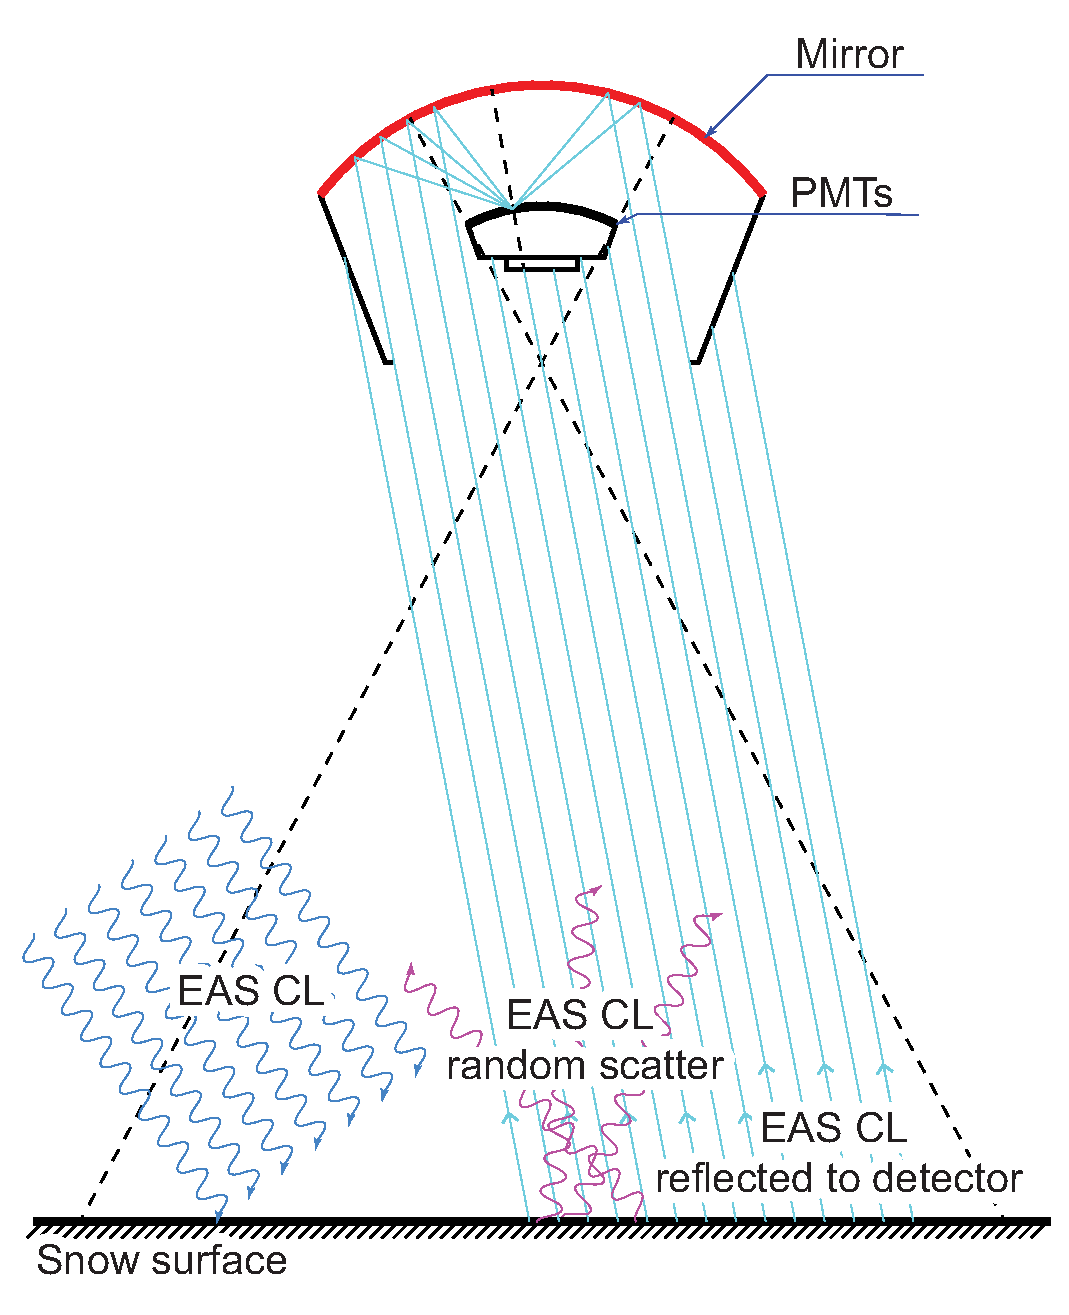
\includegraphics[width=0.42\textwidth]{optics}
    \caption{The detector optical scheme.}
\label{fig:optics}
\end{figure}

\section{The SPHERE-2 detector telemetry systems}
\label{sect:detector}

The \mbox{SPHERE-2}~\cite{Ant20} is a compact detector designed to register EAS Cherenkov light reflected from the ground snow. The detector was lifted using a tethered balloon to altitudes of up to 0.9~km above the snow covered surface. A special tethered balloon BAPA~\cite{Ant20} was developed and manufactured by the Russian Augur balloon systems agency~\cite{Augur}.

The \mbox{SPHERE-2} detector optics was comprised of a 1.5~m diameter spherical mirror with a 109 photomultiplier tubes (PMT) mosaic. The optical scheme of the detector is shown in Figure~\ref{fig:optics}.
The effective EAS registration solid angle for this scheme is about 2.2~sr, but with higher thresholds up to 3~sr.


%%%%%%%%%%%%%%%%%%%%%%%%%%%%%%%%%%%%%%%%%%%%
%%% === Statistics table === %%%
\begin{table}[tb]
\centering
\caption{The annual statistics of the SPHERE experiment on Baikal Lake. Time column lists total data taking time. The details on electronics can be found in~\cite{Ant20}.
}
\label{tab:statistics}
%\vspace{1pc}
\begin{tabular}{ccccr}
    \toprule
    year  & flights & \parbox[c]{1.5cm}{\centering{}PMT\\number}    & \parbox[c]{1.5cm}{\centering{}time,\\hours} & \parbox[c]{2cm}{\centering{}triggers\\ registered}\\ 
    \midrule
    \multicolumn{5}{c}{test runs} \\
    \midrule
    2008 & 1 &  20 &  1 &  6\,180\hspace{5mm} \\ 
    2009 & 3 &  64 & 13 & 10\,312\hspace{5mm} \\ 
    2010 & 6 &  96 & 30 &  1\,343\hspace{5mm} \\
    \midrule
    \multicolumn{5}{c}{experiment runs} \\
    \midrule
    2011 & 4 &  96 & 30 & 20\,571\hspace{5mm} \\
    2012 & 5 & 108+1 & 31 &  7\,716\hspace{5mm} \\
    2013 & 5 & 108+1 & 33 &  3\,813\hspace{5mm} \\
    \bottomrule
\end{tabular}
\end{table}
%%%%%%%%%%%%%%


The PMT mosaic was located near the mirror focal surface and recorded Cherenkov light reflected from the snow covered surface below the detector. The PMTs were arranged in a hexagonal structure on the spherical surface, see details in~\cite{Ant20} or on Figure~\ref{fig:2012-3_shore_image}. FEU-84/3 PMTs were used in the mosaic. The fields of view of the PMTs are fixed in angular terms but the exact shape and area of the snow covered surface observed by a single PMT depends on the PMT's position in the mosaic and of the altitude and orientation of the detector. The exact numbers of photomultipliers in each season are given in Table~\ref{tab:statistics}. 

The detector underwent updates and upgrades between measuring seasons that resulted in higher sensitivity in 2011 and significantly lower noise in 2012. The number of PMTs was increased to 109, the signal sampling rate was changed in 2012 from~40~MHz to 80~MHz etc. The details on electronics can be found in~\cite{Ant20}.


\subsection{Control block telemetry}

The control block of the SPHERE-2 detector contains a large set of various sensors, as well as the main recording electronics and a power supply system. Sensors located both inside and outside of the control block were used to monitor the detector state and performance and to collect supplementary data for EAS measurements. The list of sensors used, their measuring range, precision and data collection frequency is given in the Table~\ref{tab:telemetry_sensors}. 

%%%%%%%%%%%%%%%%%%%%%%%%%%%%%%%%%%%%%%%%%%%%
%%% === Telemetry table === %%%
\begin{table*}[bth]
\centering
\caption{SPHERE-2 telemetry data readout intervals and sensors precision.}
\label{tab:telemetry_sensors}

%\vspace{1pc}
\begin{tabular}{|c|l|l|c|r@{\hspace{1mm}}c@{\hspace{1mm}}l|c|}
\hline
\multicolumn{1}{|c|}{interval} & \multicolumn{1}{c|}{parameter} & \multicolumn{1}{c|}{data}  & \multicolumn{1}{|c|}{accuracy} & \multicolumn{3}{c|}{range}  & \multicolumn{1}{c|}{units} \\
%\hline
\hline
\multirow{6}{*}{1 sec} & \multirow{3}{*}{Detector position} &GPS altitude & (1)* &  -1500&--&18000  & m a.s.l.\\
                                                      \cline{3-8}
                         &                              & GPS position & 3--5 (2)* & &---&& m\\
                                                      \cline{3-8}
                       &                              & GPS time (PPS)& 1 & &---&& $\mu$s \\
                       \cline{2-8}
                       & \multirow{2}{*}{Detector orientation} & inclination angles (resolution) X,Y& 0.3 (0.02)* &$-$25&--&25&deg\\
                                                      \cline{3-8}
                       &                              & compass azimuth (resolution) Z &2.5 (0.5)* &0&--&360&deg\\
                       \cline{2-8}
                       &Control block                 & inner temperature& 1.5 & $-40$&--&70 &$^\circ$C\\
\hline
\multirow{7}{*}{1 min} & \multirow{2}{*}{PMT status} & anode current & 0.03 & 0&--&125 & $\mu$A\\
                                                      \cline{3-8}
                       &                              & mosaic temperature & 1.5 & $-40$&--&70 & $^\circ$C\\
                       \cline{2-8}
                       & Power source                 & high voltage (HV1) & 0.1 & 0&--&250 & V\\
                       \cline{2-8}
                       & \multirow{2}{*}{Barometer}   & pressure & 5 & 750&--&1100 & hPa\\
                                                      \cline{3-8}
                       &                              & temperature& 2 & -20&--&60 &$^\circ$C\\
                       \cline{2-8}
                       & Balloon barometer            & pressure   & 3 & 0&--&1000 & Pa\\
                       \cline{2-8}
                       & Battery (19V)                & voltage & 0.01 & 0&--&40 & V\\
                       \cline{2-8}
                       & Constant voltage (5V)        & voltage & 0.01 & 0&--&40 & V\\
\hline
\multirow{5}{*}{10 min} & \multirow{3}{*}{PMT status} & first dinode voltage & 0.06 & 0&--&250 & V\\
                                                      \cline{3-8}
                       &                              & PMT temperature & 0.1 & -30 &--&50 & $^\circ$C\\
                                                      \cline{3-8}
                       &                              & supply voltage & 0.006 & 0&--&25 & V\\
                       \cline{2-8}
                       & Trigger                      & counting rate & -- &0&--&65536& \\
                       \cline{2-8}
                       & FADC boards                  & voltage (1.2, 2.5, 2.8) & 0.001 & 0&--&4 & V\\
\hline
\end{tabular}

\vspace{1mm}

\footnotesize \raggedright 
\hspace{5 mm}* numbers in parentheses are given according to our own analysis (see in Section~\ref{sect:orientation})
%2 m accuracy according to the manufacturer provided data, 
%1 m accuracy according to our own analysis (see in Section~\ref{sect:orientation} )
%\hspace{5 mm}**  3–5 meters, 95\% typical accuracy according to the manufacturer provided data, 2 m accuracy according to our own analysis (see in Section~\ref{sect:orientation} )
\normalsize
\end{table*}

%%%%%%%%%%%%%%%%%%%%%%%%%%%%%%%%%%%%%%%%%%%%

%The sensors inside the control block measured:
%\begin{itemize}[nosep]
%\item temperature of the FADC boards by two sensors per board for cooling system operation;
%\item voltage on the secondary power supply units for PMT mosaic power stabilization;
%\item voltage and current on the main power supply unit;
%\item overpressure and temperature inside the balloon.
%\end{itemize}
%The sensors outside the control block measured:
%\begin{itemize}[nosep]
%\item detector position (GPS-module);
%\item local air pressure and temperature;
%\item horizontal orientation (compass).
%\end{itemize}
%Additional sensors were installed on the PMTs in the mosaic and controlled
%\begin{itemize}[nosep]
%\item power supply voltage;
%\item anode current;
%\item temperature.
%\end{itemize}

Some of the sensors were located inside the control block, some outside on the surface (like GPS and pressure sensor), some on the PMT mosaic (inclinometer, compass, PMT current and voltage sensors etc.). See~\cite{Ant20} for details.

Some of the data provided by these sensors was used to monitor the flight conditions and detector status in real time. Also, all of the data was stored and later used in EAS parameters reconstruction and detector performance evaluation.

\subsection{Orientation control system}
\label{sect:orientation}

At the rest state the detector axis was oriented vertically and the detector observed the snow covered surface just under itself. During the measurements the detector was hung under the balloon and swung and rotated freely. Its inclination is an important factor for shower parameter reconstruction since it determines the overall geometry of the experiment. To control the position and rotation of the detector a dual-axis inclinometer and a digital compass were installed on the PMT mosaic control board. 

The compass measured the angle of the detector's orientation relative to the Earth's magnetic field with a 2.5~degree precision.

The inclinometer measured two angles between its internal orthogonal axes and the plane orthogonal to the gravity vector. The orientation of the inclinometer's axes with respect to detector mosaic axes was determined in the laboratory. After careful preparations the mosaic was set horizontally with precision better than $0.5^\circ$ and the zero level of the inclinometer was measured. All detector inclination angles were calculated considering the recovered zero level.

The type of inclinometer used allows fast angle measurements with low power consumption, but, unlike the gyroscopic ones, it is affected by acceleration. As we will see in Section~\ref{sect:telemetrydata} during the experimental measurements there was recorded only a single instance of strong wind gusts at the end of the 2013-3 flight, and the balloon position was relatively stable at all other times. So we assumed that the registered inclination angles were unaffected by swinging.

The Garmin 16xHVS~\cite{GPS-module-specs} GPS sensor, located on the control unit, was used to measure geographical coordinates and elevation above sea level. The GPS manufacturer declared a 3–5 meters, 95\% typical accuracy in position measurements.
%, and 2~m accuracy in the altitude determination. 
Our observations show that the accuracy of position detection by the GPS sensor differed for moving and stationary situations. 

The accuracy of the GPS sensor in stationary state was calculated from GPS data when the detector was stationary on the ice. Daily distributions of the detector position and altitude were plotted for 20 days in 2012 and 2013. The median sigma of these distributions was taken as the accuracy of the position and altitude measurements: 2~m and 1~m respectively.

However, the GPS detector showed a significant lag in altitude measurements during the initial balloon climb and subsequent flight altitude changes. More details on this lag, its correction and influence on detector altitude determination are discussed in Section~\ref{sect:gps_correction}.

%%%% Какая есть телеметрия %%%%%

\subsection{Telemetry monitoring\label{sect:telemetry}}

During every experimental flight a lot of information about the detector status and environmental parameters was recorded. Various telemetry data was received and checked every second, every minute, and every 10 minutes as shown in the Table~\ref{tab:telemetry_sensors}.

Every second the detector position and orientation was recorded. The GPS data (altitude, latitude, and longitude), universal global time UTC, the angles of detector inclination, digital compass data and the control block inner temperature was monitored. An additional GPS and barometer were located in the control booth at ice level.

Every minute the PMT and power status were monitored: anode currents of each PMT, the PMT mosaic temperature, the temperature of the PMTs high voltage power source, power supply voltage and DC voltage sources were recorded. Barometer sensors were also polled every minute.

Every ten minutes the detector logged the PMTs supply voltages, voltages at PMTs first and tenth dynodes, individual PMT temperatures, the measuring channel counting rates and voltage on the FADC boards.

The PMTs power supply data was later used to control the operational stability of the optical modules. The registered discriminator triggering rate was used for discriminator thresholds selection in experimental flights. Deviations in power consumption by FADC boards were used to monitor possible malfunctions in the detector electronics. Data from temperature sensors was used for in-flight detector state and cooling system control.


\section{Experimental conditions}
%\section{Site and weather}
\label{sect:data}
 
The SPHERE experiment was carried out on the Baikal Lake during winter seasons of 2008--2013. The Baikal lake ice thickness reaches 40--60~cm in February and can hold heavy vehicles. The balloon launch pad was deployed on the lake surface around 700~m from the shore (near 51$^\circ$\,47'\,48''~N, 104$^\circ$\,23'\,19''~E).
%51.796923~N, 104.388663~E http://www.google.com/maps?q=51.796923,+104.388663

The \mbox{SPHERE-2} detector was lifted by a tethered balloon BAPA to altitudes of up to 900~m above the snow covered surface. The annual statistics of the experiment are given in Table~\ref{tab:statistics}. The first three years were dedicated to test runs. 

%Unless otherwise specified, all illustrations in the paper are given for the \mbox{SPHERE-2} data of the winter 2013 run. All plots were made with the Python Matplotlib plotting library.

\subsection{Weather and snow}

Measurements were carried out during clear moonless nights with low wind conditions. The measurements were started 1.5 hours after sunset or immediately after moonset and finished before moonrise or 1.5 hours before sunrise. If the wind conditions became unsuitable for the flight of the balloon, the detector was landed at once. However, this happened only once during the third flight in 2013. The typical night air temperature on the lake surface was near $-15$~$^\circ$C. According to the \href{https://rp5.ru/Weather_in_the_world}{Reliable Prognosis} data archive~\cite{rp5} from the nearest weather stations 30818 and 30710 the horizontal visibility was `at least 10 km' (the highest possible grade in the system), and the altitude of the base of the lowest clouds was `2500~m or more or no clouds present' (the best transparency that these stations can measure).

Our own observations of the atmosphere show that during the day the visibility degraded due to high humidity (as is the case shown in Figure~\ref{fig:baikal_snow}), but in the evening recovered back. In~Figure~\ref{fig:baikal_atmo} the background mountains are 55--56~km away therefore the horizontal visibility was good. In the nights the mountains were also visible. The Milky Way was clearly visible during all measurement nights. 

Another atmosphere property that was monitored during measurements was its density. The optical transparency is a crucial property for Cherenkov light reliant methods of EAS studies since it directly influences the measured light fluxes and later the primary particle energy estimations. However, the atmosphere density profile is also vital for the primary particle type studies since it affects the altitude of shower development and its Cherenkov light lateral distribution. The influence of the selected atmosphere on the Cherenkov photons lateral distribution and its properties are discussed below in Section~\ref{sect:atmosphere-profile}.

The atmosphere density profile was reconstructed based on air pressure and temperature measurements during the initial climb in the beginning of the night and during the descent at the end. During almost all measurement nights the atmosphere remained stable. Stable atmosphere conditions were expected due to the known Siberian High phenomena. However, during two flights 2012-3 and 2013-5 a rapid change in the atmosphere profile was observed (see Figure~\ref{fig:density}) followed by rapid weather worsening (clear sky changed to cloudy, wind became stronger with gusts), which, unfortunately, is indicative of the climate change and observed weakening of the Siberian anticyclone. 

%% Baikal snow photo %% fig:baikal_snow
\begin{figure}[tb]
\begin{center}
    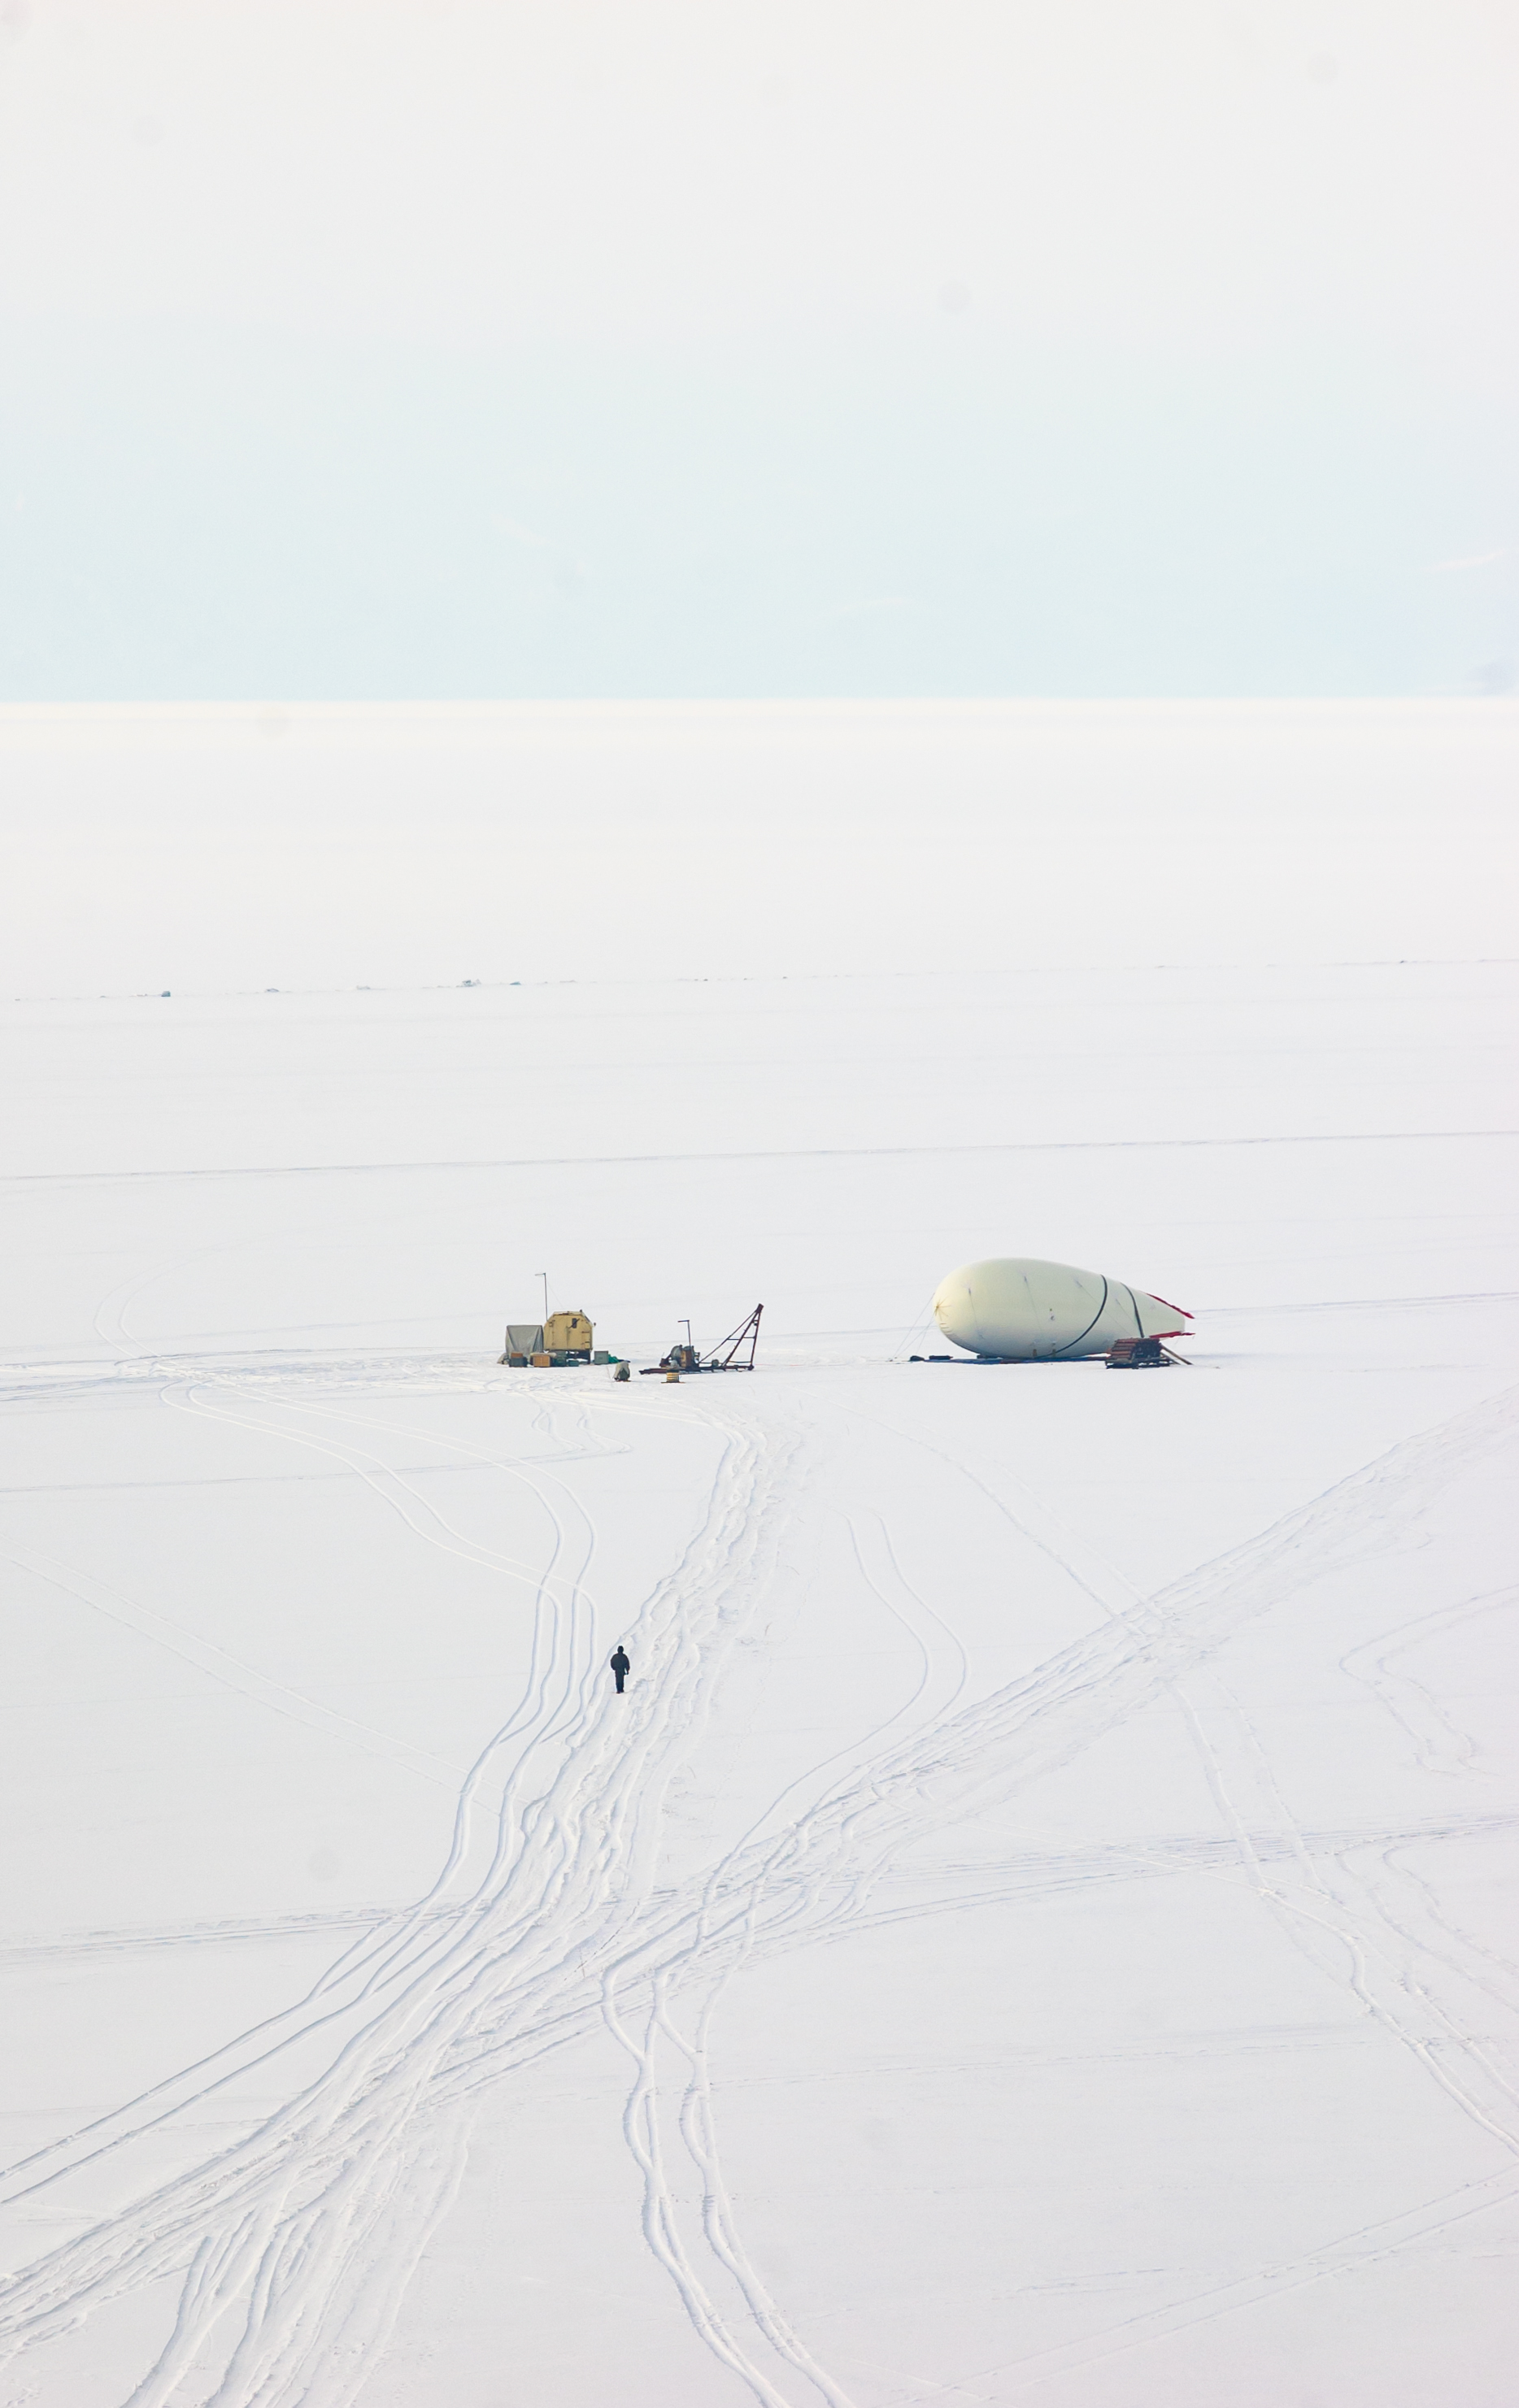
\includegraphics[trim=1cm 5cm 0cm 5cm,clip,width=0.45\textwidth]{DSC_4049.jpg}\hspace{2pc}%
    \caption{An overview of the launch site on the Baikal Lake from a hill on the shore. The snow coverage around the SPHERE start point was thick and usually renewed between flights by occasional snowfalls.}
\label{fig:baikal_snow}
\end{center}
\end{figure}


\begin{figure}[tb]
\begin{center}
    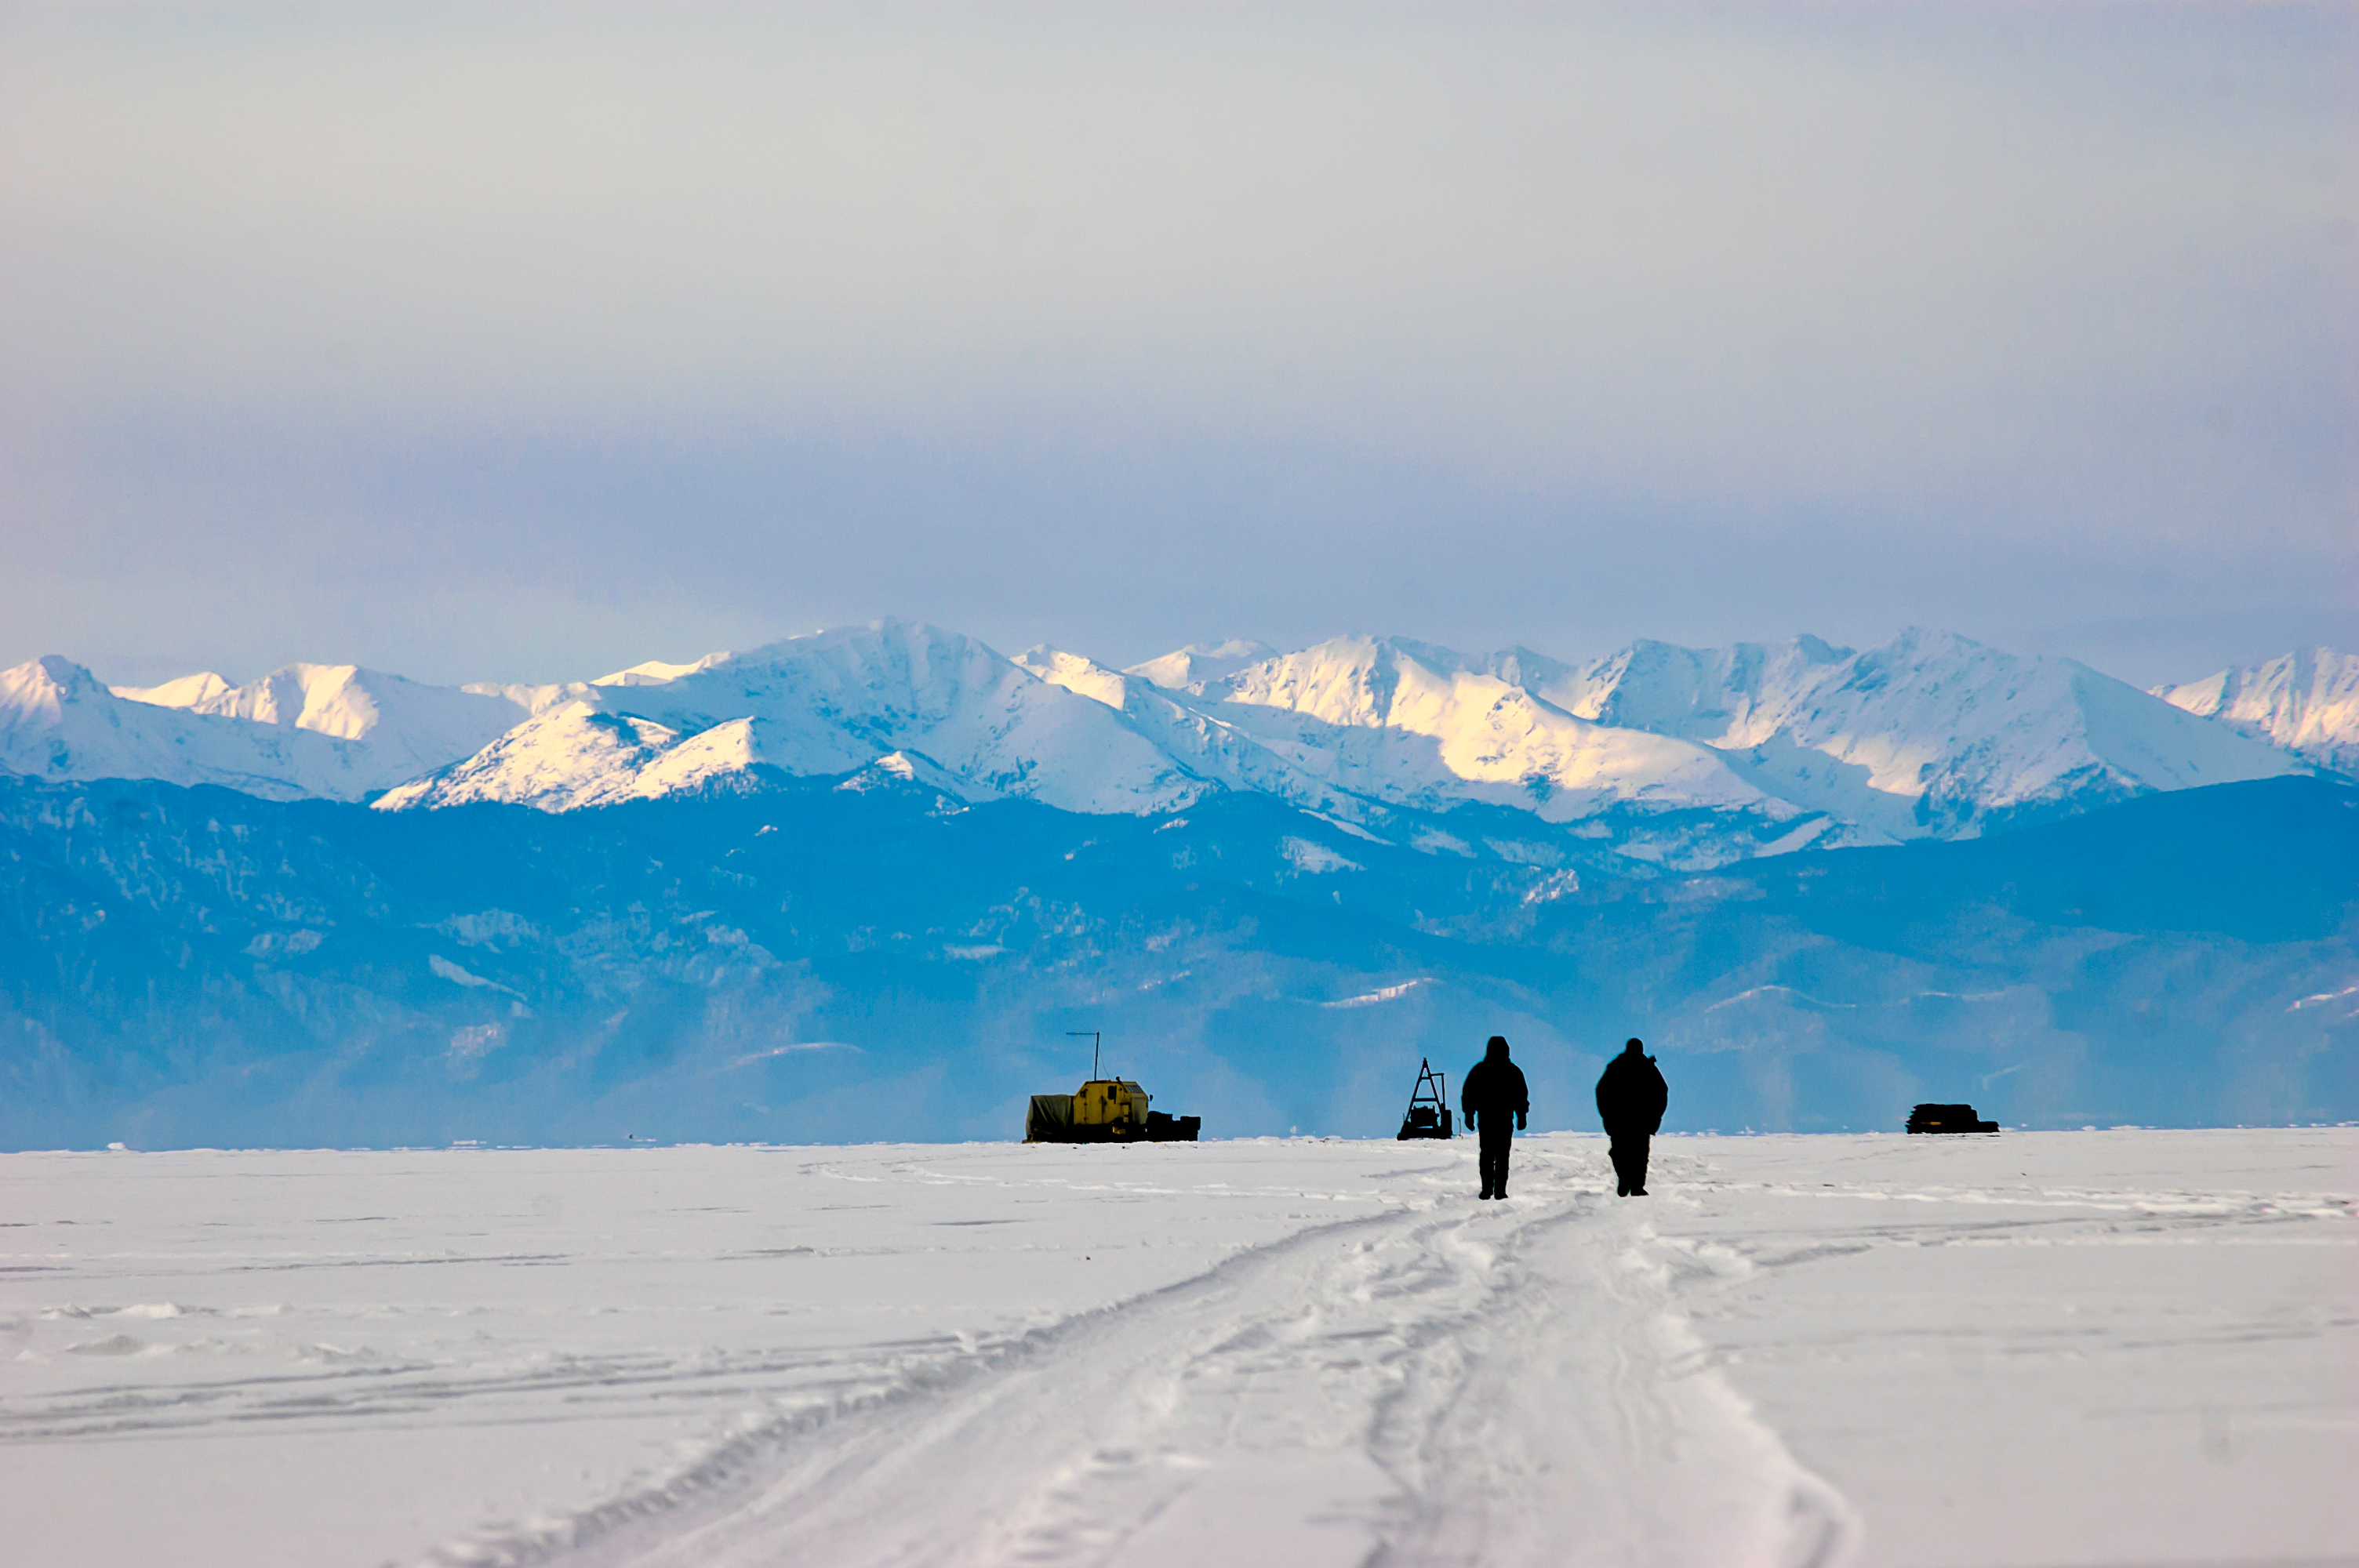
\includegraphics[width=0.45\textwidth]{DSC_7423.jpg}\hspace{2pc}%
    \caption{An overview of the launch site on the Baikal Lake from the shore. The background mountains are more than 50 kilometers away which indicates good atmosphere transparency on ground level.}
\label{fig:baikal_atmo}
\end{center}
\end{figure}


The measurements were performed at the end of winter season when the Baikal lake was covered with thick ice. The snow coverage of the ice differs from year to year and in different areas of the lake according to prevailing winds. However in winters 2010--2013 the lake area near the launch site was covered with a thick (up to 40~cm) layer of snow with occasional snowfalls. In Figure~\ref{fig:baikal_snow} the snow coverage in 2012 is shown. This was the typical coverage during all measurements. The snow reflection properties were controlled using a photometer. The influence of the snow state on its reflecting properties has been discussed in detail in our article on the simulation of the SPHERE-2 detector~\cite{Ant19}.


%%%%%%%%%%%%%%%%%%%%%%%%%%%%%
%% Figure 4  detector drift figure  %%%
%%% fig:gps-compass
\begin{figure}[tb]
    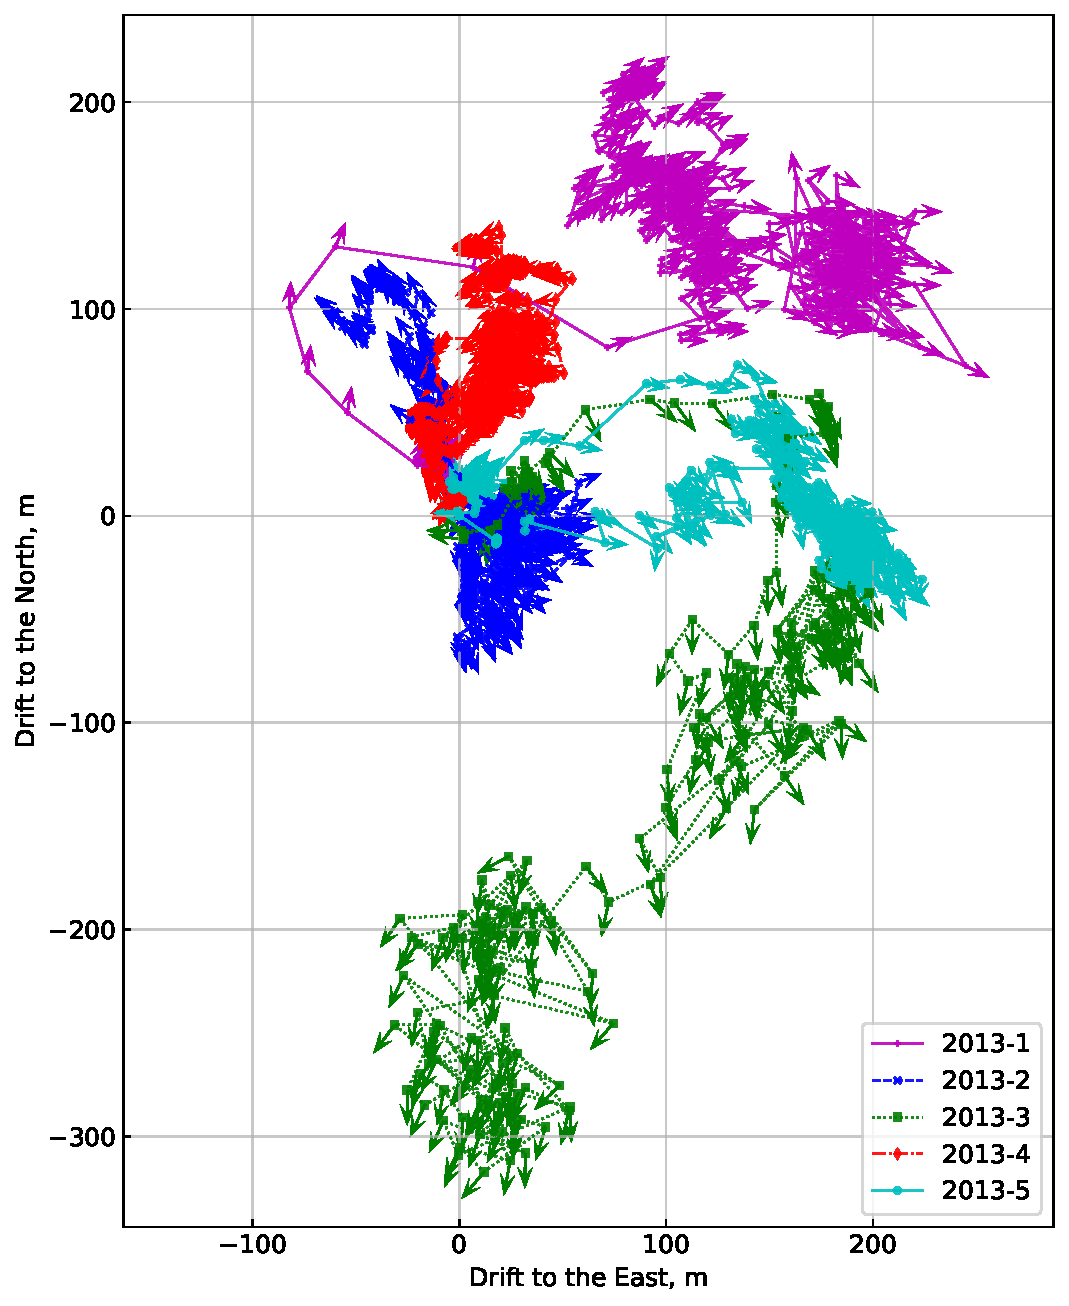
\includegraphics[width=0.45\textwidth]{figs/fig4_GPS_drift.pdf}\hspace{2pc}%
    \caption{The SPHERE-2 detector drift in 2013. The arrows indicate the detector magnetometer orientation. The start point is located at zero coordinates. The points indicate detector position in 1 minute intervals.}
\label{fig:gps_compass}
\end{figure}
%%%%%%%%%%%%%%%%%%%%%%%%%%%%%

 
\subsection{Detector orientation and telemetry data}
\label{sect:telemetrydata}

The \mbox{SPHERE-2} detector's position and inclination depend on wind conditions near the detector, see Figure~\ref{fig:gps_compass} and Figure~\ref{fig:inclination}. In Figure~\ref{fig:gps_compass} the position of the detector with the magnetometer data is shown for the 2013 season  flights. The position was reconstructed using GPS data with the launch point being located at zero coordinates. The detector orientation measured by the magnetometer is indicated by arrows. Figure~\ref{fig:gps_compass} demonstrates that wind was quite constant during most of the time and the balloon position was rather stable and varied slowly.  

%%%%%%%%%%%%%%%%%%%%%%%%%%%%%
%%  4 telemetry  pictures %%%
%% Figures 5 and 6 
\begin{figure*}[tb]
    \begin{minipage}[t]{0.48\textwidth}
       \centering
       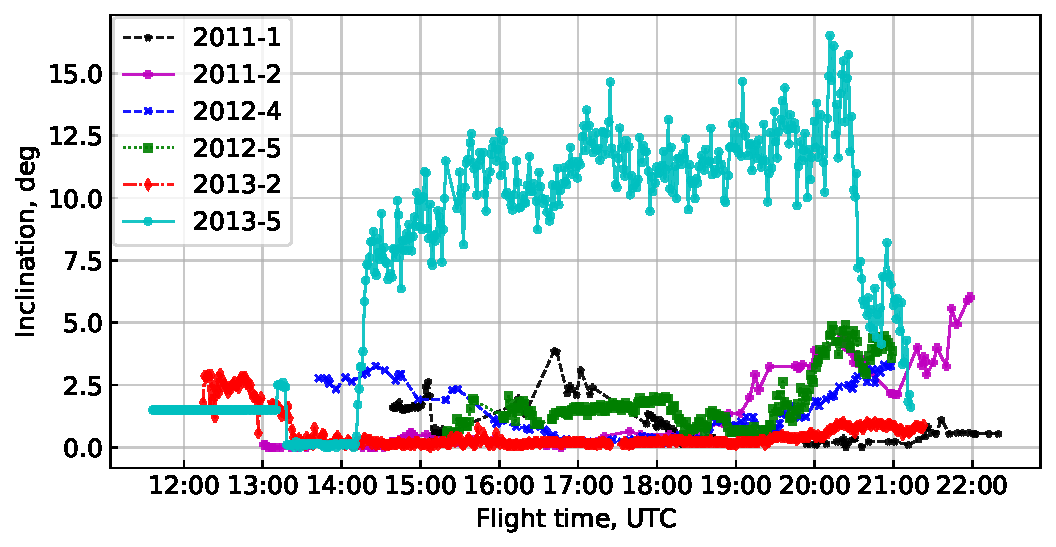
\includegraphics[width=\textwidth]{Telemetry_inclination.pdf}
       \caption{The detector inclination according to the inclinometer sensor during several flights in 2011-2013.}
       \label{fig:inclination} 
    \end{minipage}
    \hfill
    \begin{minipage}[t]{0.48\textwidth}
       \centering
       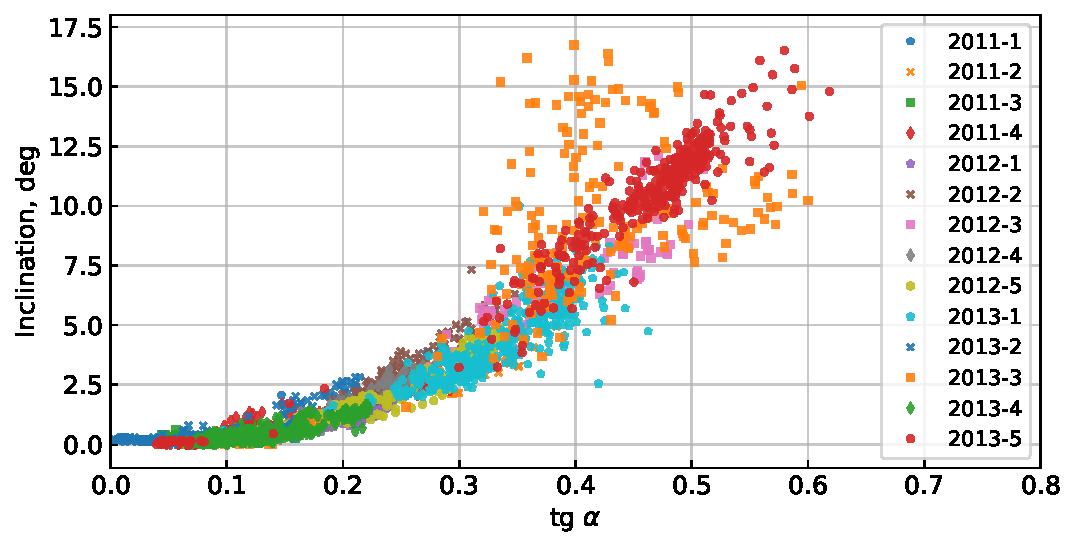
\includegraphics[width=\textwidth]{tg-inclination.pdf}
       \caption{Detector inclination against the detector drift from the start point to the detector altitude ratio which roughly translates into the tether inclination angle. See text for details on detector behavior.}
       \label{fig:drift-inclination}
   \end{minipage}
\end{figure*}
%%%%%%%%%%%%%%%%%%%%%%%%%%%%%   
%%%%%%%%%%%%%%%%%%%%%%%%%%%%%
%% Figures 7 and 8
\begin{figure*}[tb]    
    \begin{minipage}[t]{0.48\textwidth}
        \centering
        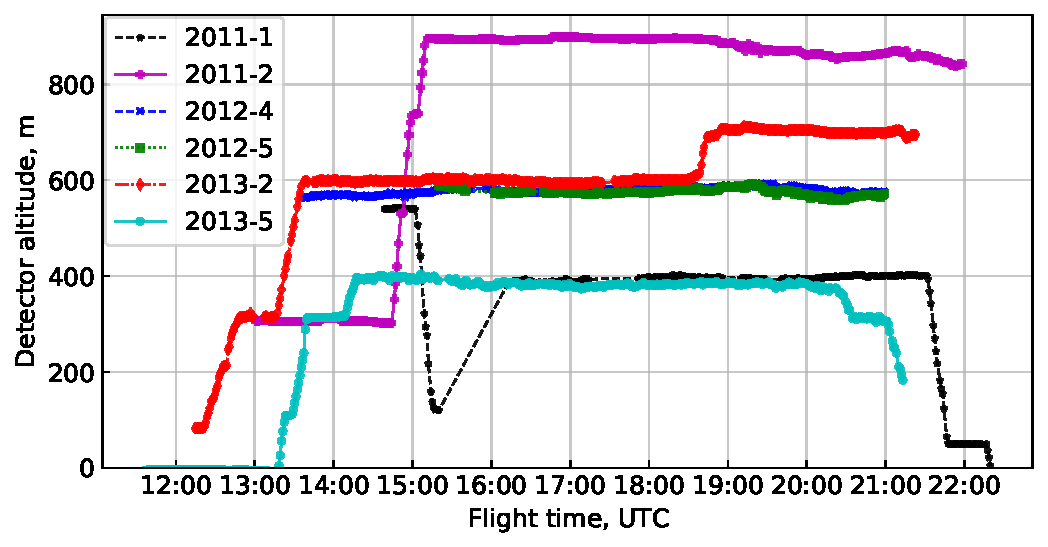
\includegraphics[width=\textwidth]{Telemetry_height.pdf}
        \caption{Altitude of the SPHERE-2 detector carried by the BAPA tethered balloon according to the GPS module data during 2011--2013 flights.}
        \label{fig:height}
    \end{minipage}
    \hfill
    \begin{minipage}[t]{0.48\textwidth}
        \centering
        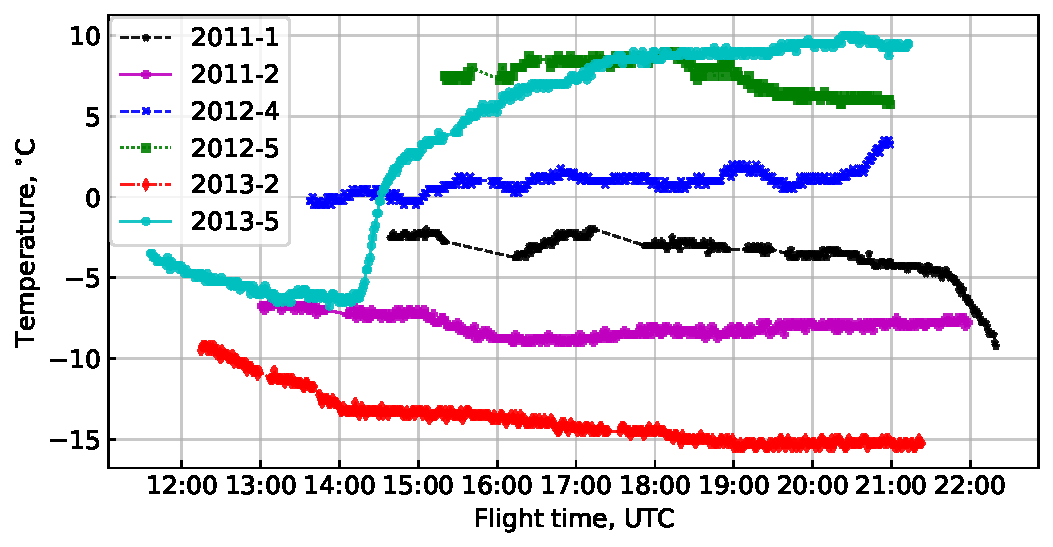
\includegraphics[width=\textwidth]{Telemetry_tmos.pdf}
        \caption{Air temperature near the PMT mosaic during 2011--2013 runs.}
        \label{fig:temperature}
    \end{minipage}
\end{figure*}
%%  4 telemetry  pictures %%%
%%%%%%%%%%%%%%%%%%%%%%%%%%%%%


%%%%%%%%%%%%%%%%%%%%%%%%%%%%%
%% Figures 9 and 10
\begin{figure*}[tb]    
    \begin{minipage}[t]{0.48\textwidth}
        \centering
        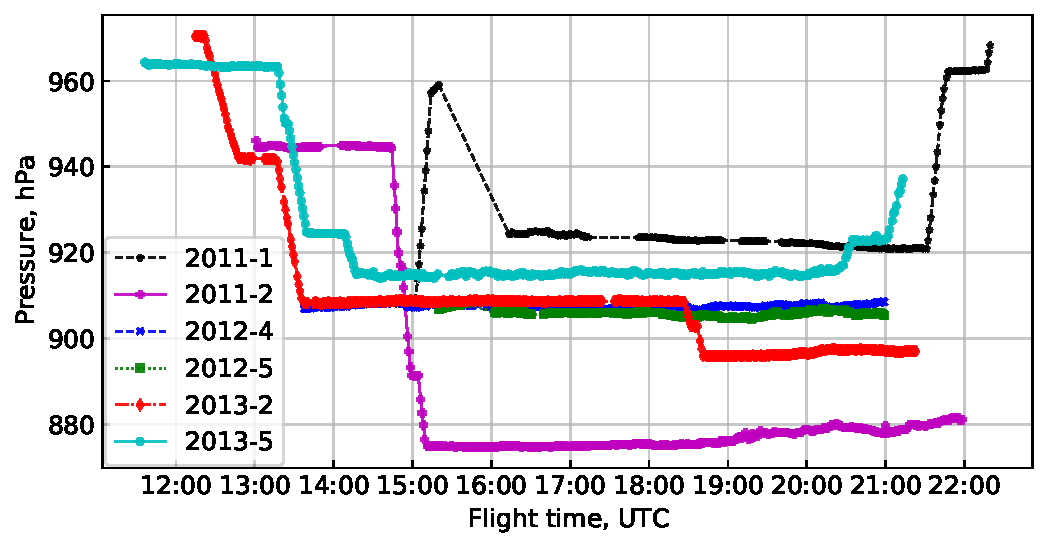
\includegraphics[width=\textwidth]{Telemetry_pressure.pdf}
        \caption{Air pressure according to the barometer sensor data during 2011--2013 flights.}
        \label{fig:pressure}
    \end{minipage}
    \hfill
    %% The central PMT current %%
    \begin{minipage}[t]{0.48\textwidth}
        \centering
        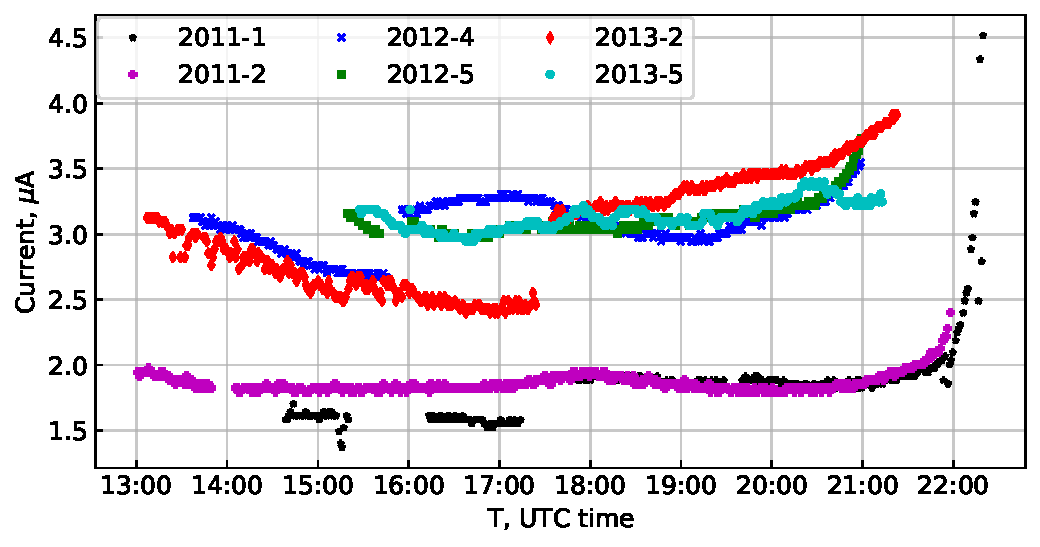
\includegraphics[width=\textwidth]{hv-53.pdf}
        \caption{The central PMT currents in different flights.}
        \label{fig:current}
    \end{minipage}
\end{figure*}
%%%%%%%%%%%%%%%%%%%%%%%%%%%%%
%%%%%%%%%%%%%%%%%%%%%
However, due to the construction of the suspension system to the balloon the detector was deflected by the wind to a certain degree in the corresponding direction away from the launchpad. In Figure~\ref{fig:inclination} the inclination of the detector is shown for some flights of the 2011--2013 runs. During some of the flights the detector was in a nearly vertical position (2011-1 or 2013-2), while in the others (2013-5) it was tilted to a significant angle. However, this declination was steady and varied slowly over time. The maximum inclination angle recorded was about 20$^\circ$. In Figure~\ref{fig:drift-inclination} the dependence of the detector inclination angle from the ratio of the drift distance from the starting point to the flight altitude (roughly the tangent of the balloon tether angle) is shown for all experimental flights. This ratio, as expected, indicates wind strength which, in turn, defines the inclination angle. Strong fluctuations in flight 2013-3 (orange squares) occurred near midnight and coincided with a rapid change in the atmosphere profile and weather worsening, which resulted in early detector landing due to bad flight conditions. The detector inclination had a significant impact on the experiment `geometry' and was taken into account at the stage of EAS parameters reconstruction.

Detector altitude above the lake surface according to the GPS data is shown in Figure~\ref{fig:height}. The GPS module had some specific properties that resulted in several minor corrections in the altitude (detailed description see below in Section~\ref{sect:gps_correction}). The surrounding air temperature and pressure that were monitored for the control of atmospheric properties are presented in Figure~\ref{fig:temperature} and Figure~\ref{fig:pressure} respectively. Detailed description of the real atmosphere profile and overview of its impact on the data analysis is given below in Section~\ref{sect:atmosphere-profile}.



\subsection{PMT currents variations}

%%%%%%%%%%%%%%%%%%%%%%%%%%%%%%%%%%%%%%%%%%
%% 2012-3 currents
%% Figures 11 and 12
\begin{figure*}[tb]
    \begin{minipage}[t]{0.48\textwidth}
        \centering
        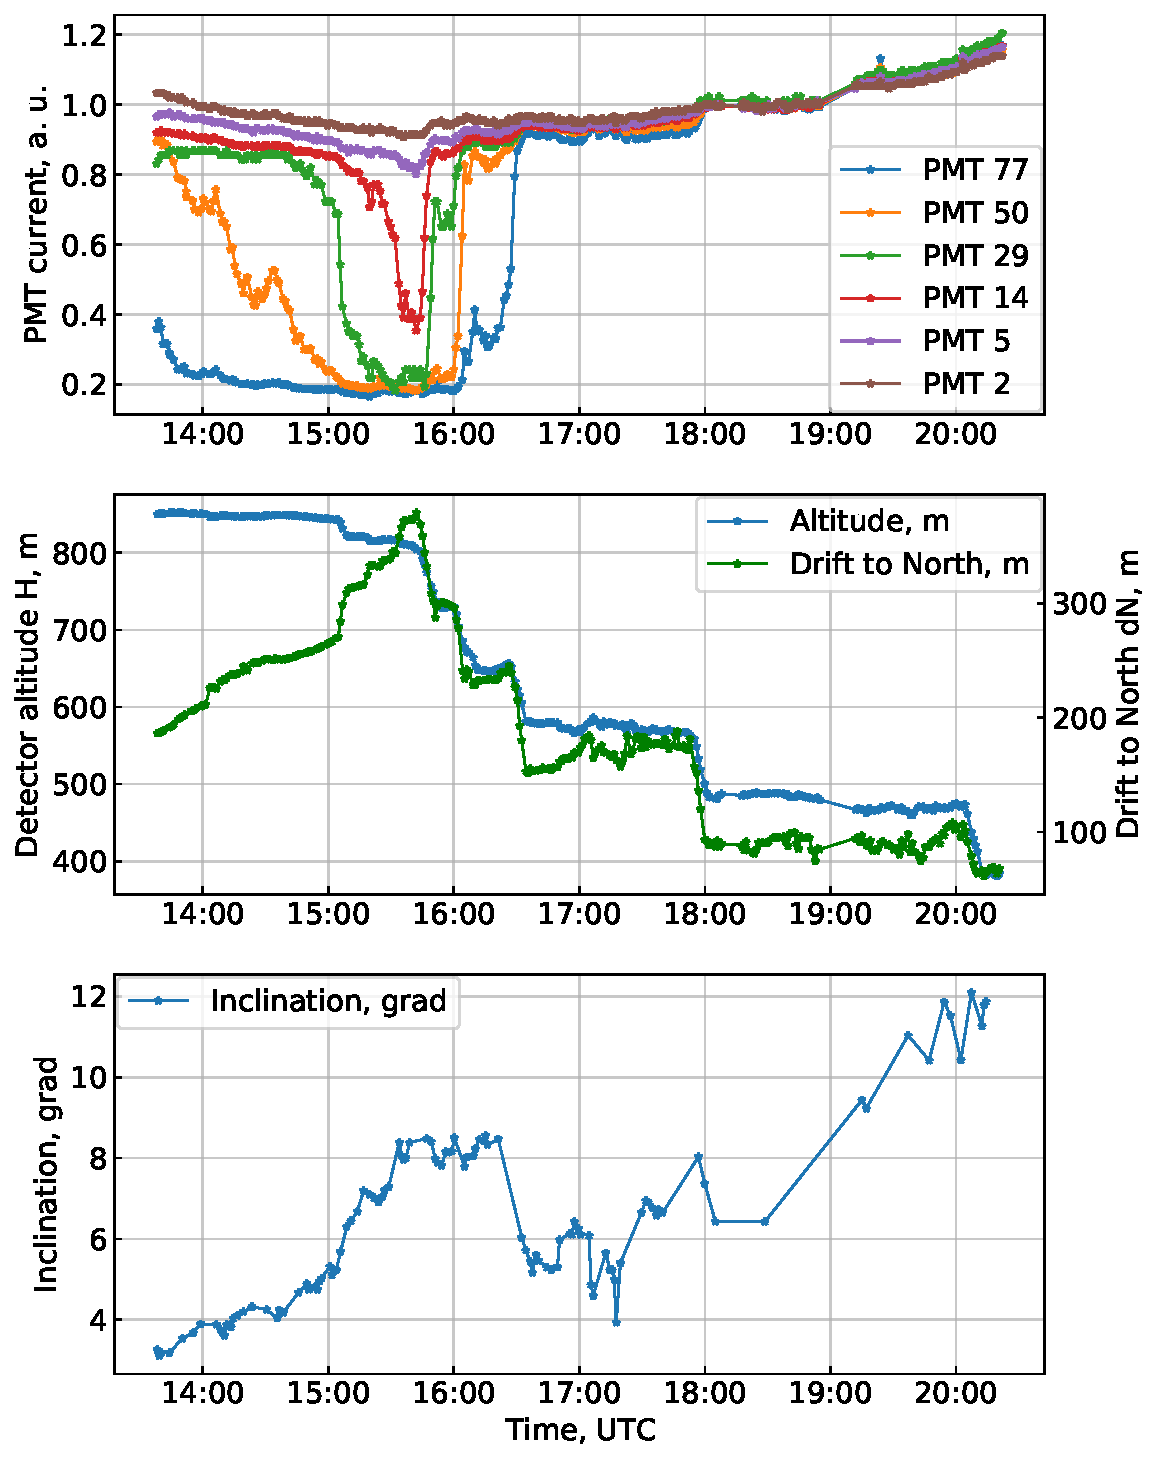
\includegraphics[width=\textwidth]{2012-3_currents_H_dN.pdf}
        \caption{PMT currents, detector altitude, drift to the North, compass and inclination during flight 2012-3.}
        \label{fig:2012-3_currents}
    \end{minipage}
    \hfill
    \begin{minipage}[t]{0.48\textwidth}
        \centering
        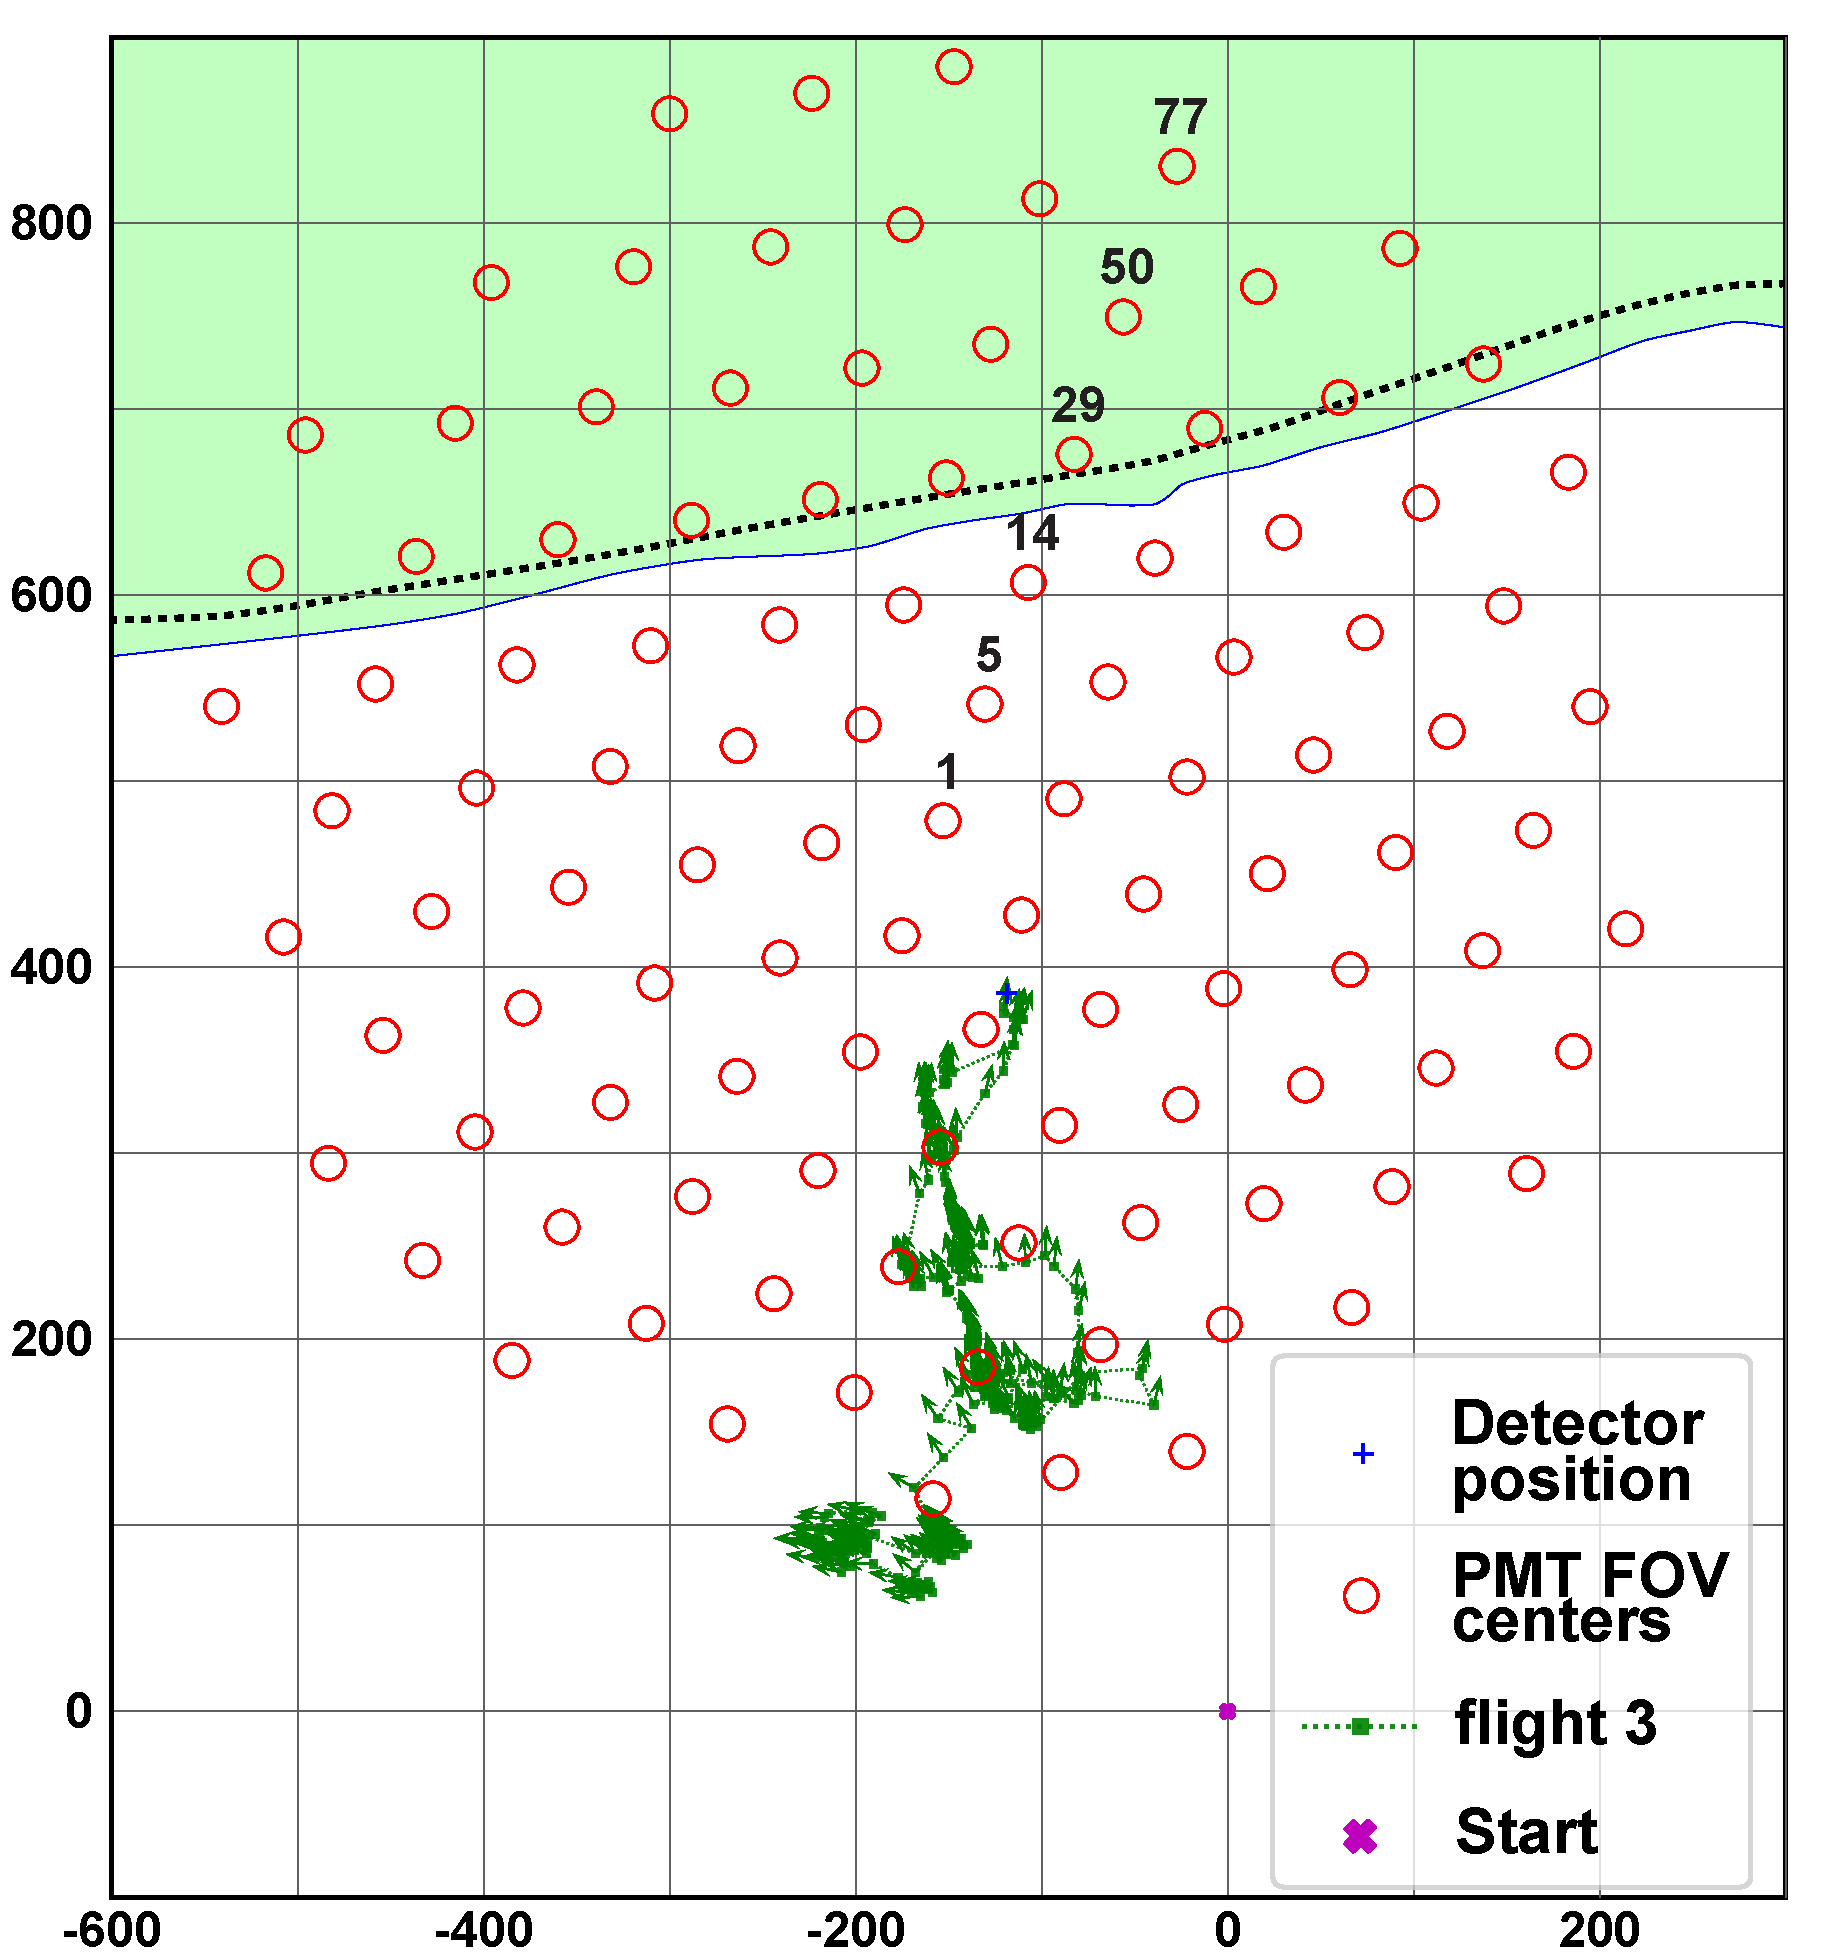
\includegraphics[width=\textwidth]{2012_drift-mod.pdf}
        \caption{The SPHERE-2 detector drift in 2012-3 flight. Mosaic projection to the show surface is given for the time 15:47 UTC. Detector GPS position at that moment is indicated by the cross.}
        \label{fig:2012-drift}
    \end{minipage}
\end{figure*}
%%%%%%%%%%%%%%%%%%%%%%%%%%%%%%%%%

 Figure\ref{fig:current} shows the anode current of the detector mosaic central PMT for some of the flights. In 2008--2011 seasons in the central position of the mosaic a FEU 84-3 PMT was used and in the seasons 2012--2013 --- a Hamamatsu R3886 PMT. The latter has a larger photocathode and amplification. Also for each flight the voltage on the PMTs was set independently and in some cases was changed mid-flight. The current increase during the last minutes of 2011 flights was due to an increase in the illumination at sunrise. In subsequent seasons the measurements were conducted at earlier dates so the sun rose later and did not affect the measurements. In general, the PMTs current variations during the observations followed the variation of the background illumination of the snow.


\begin{figure}[tb]
    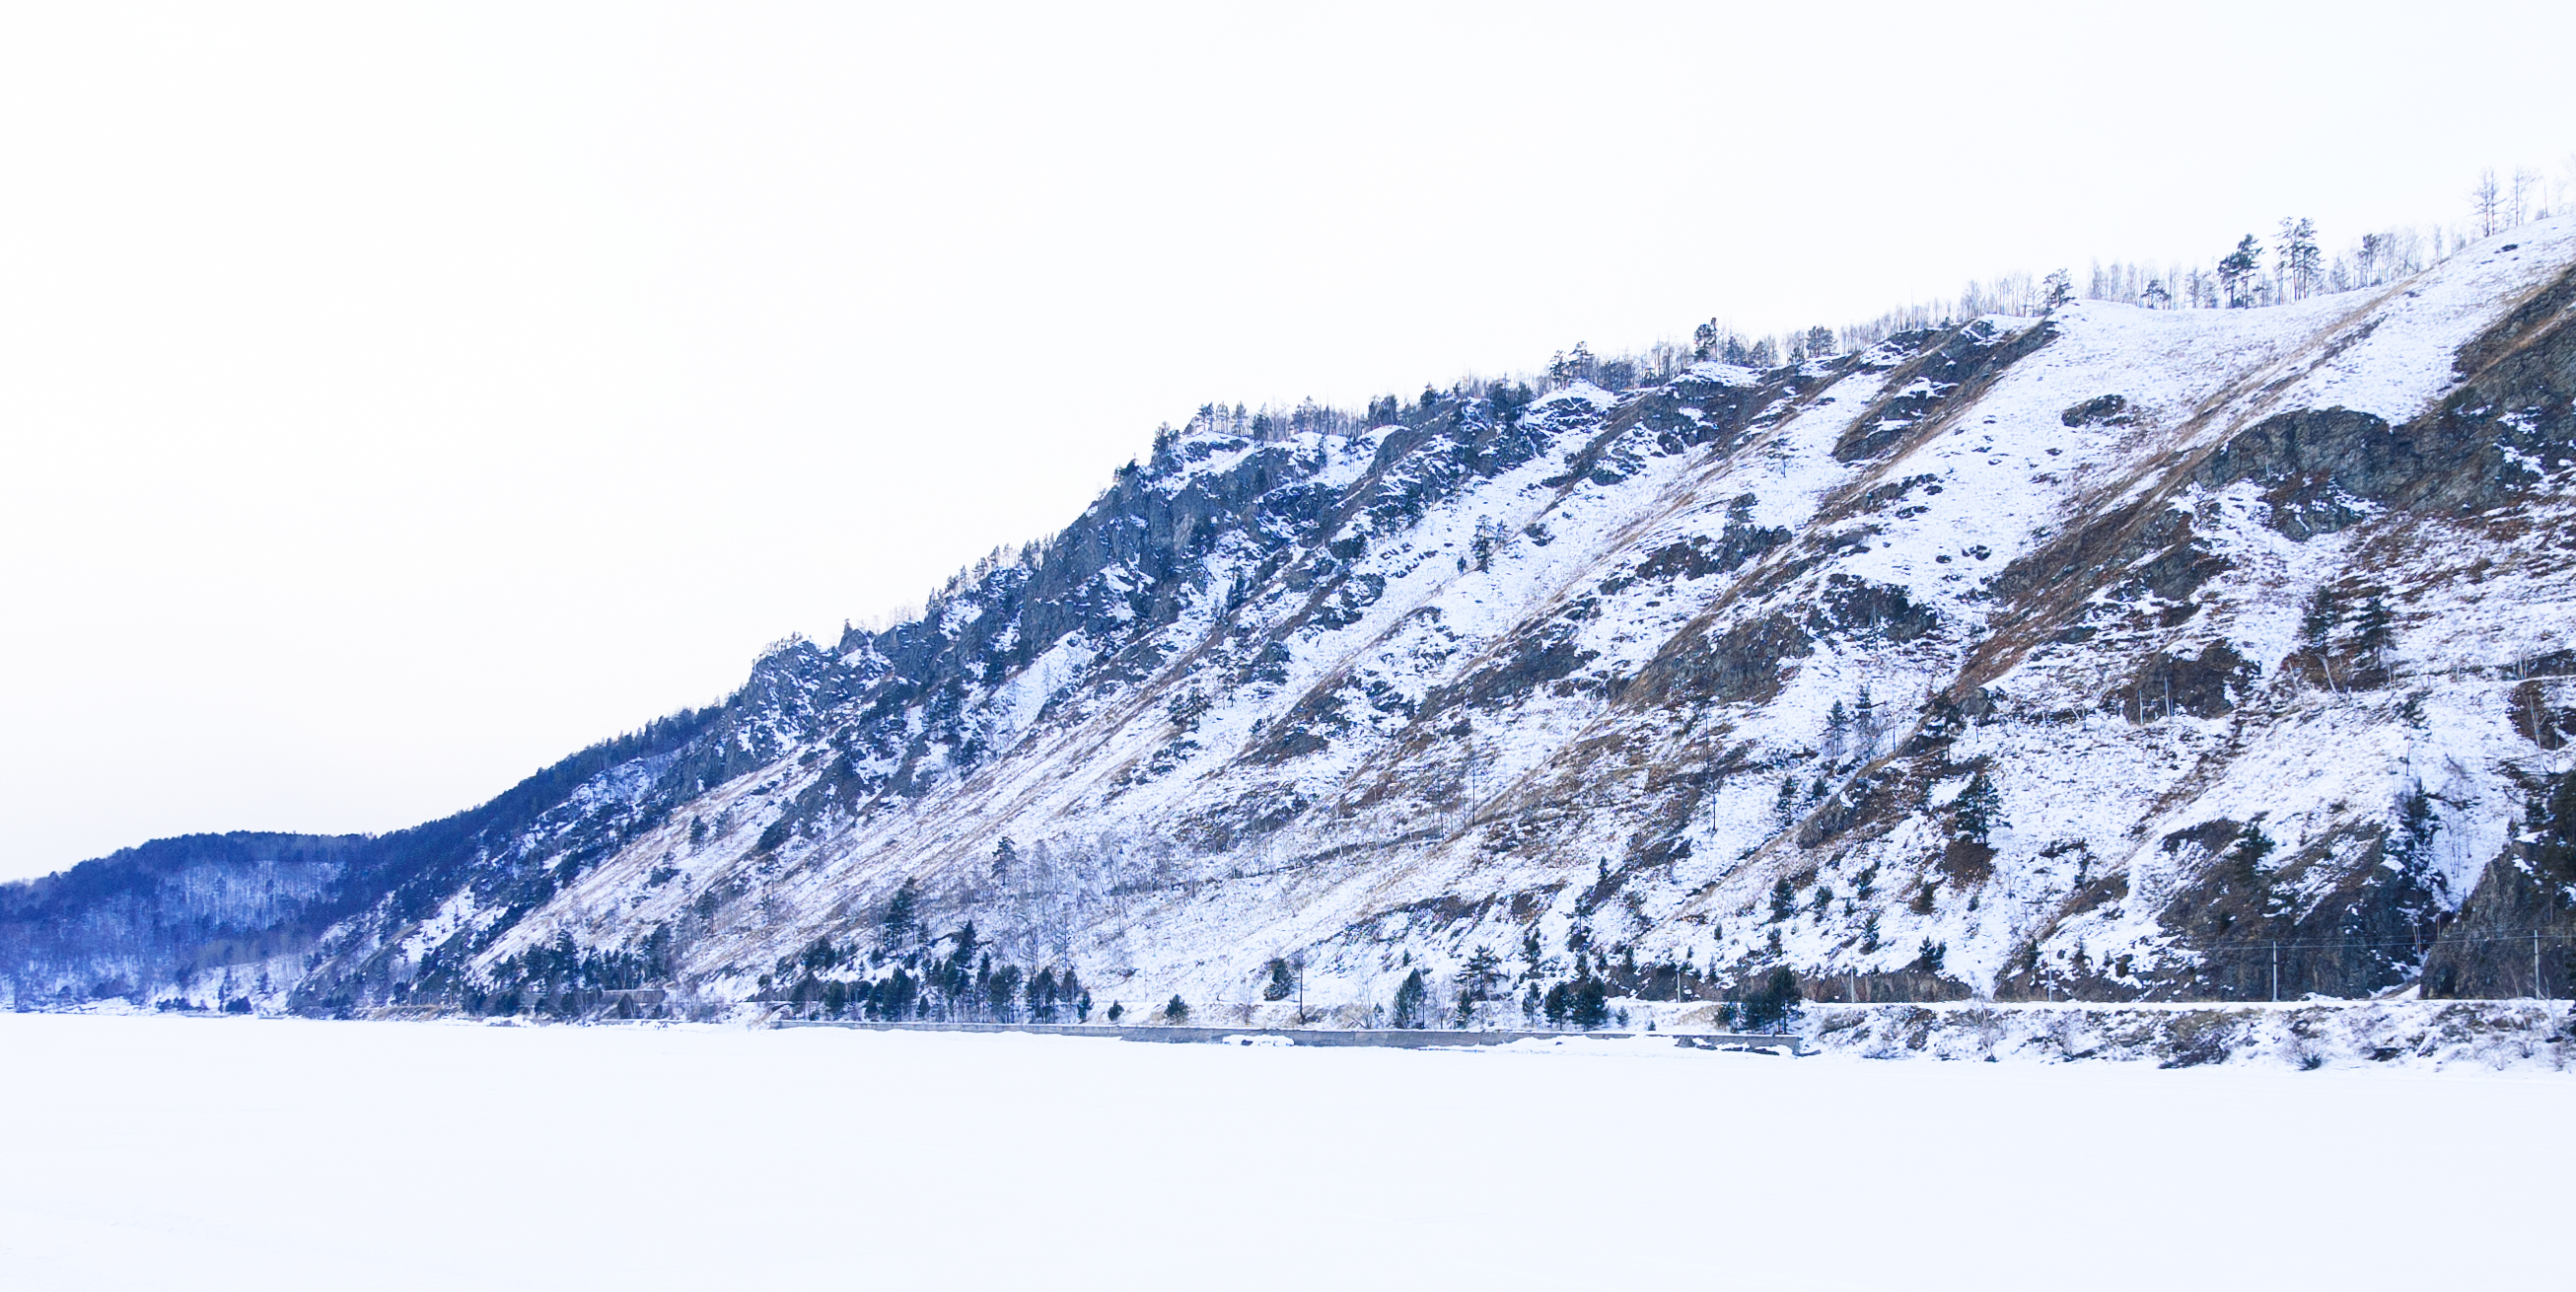
\includegraphics[width=0.48\textwidth]{DSC_7256_1.jpg}
    \caption{View on the shoreline Section `observed' by the detector from the position indicated on Figure~\ref{fig:2012-drift} is in the middle of the photo.}
    \label{fig:2012--shore-view}
\end{figure}
%%%%%%%%%%%%%%%%%%%%%%%%%
%%%%%%%%%%%%%%%%%%%%%%%%%
\begin{figure}[tb]
\centering
    %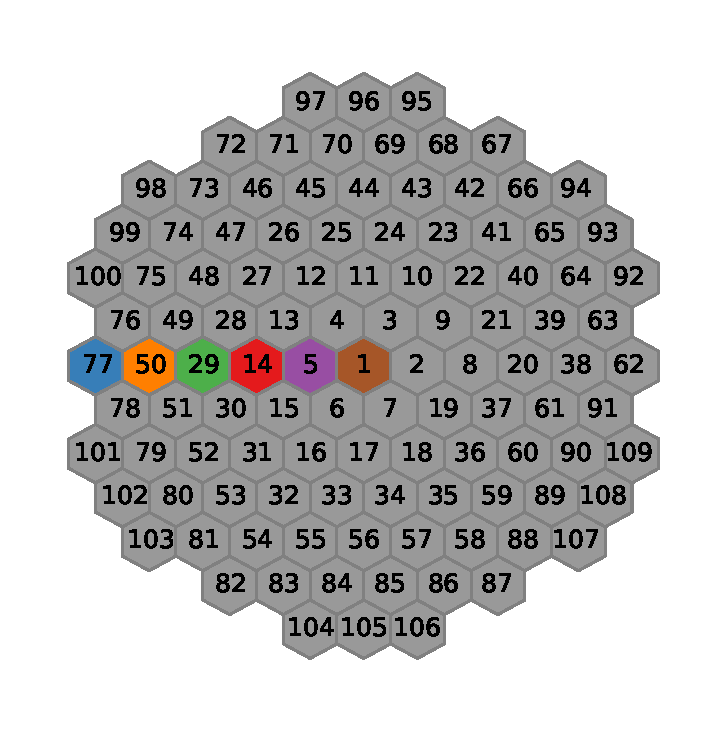
\includegraphics[width=0.2\textwidth]{2012-3_retina.pdf}
    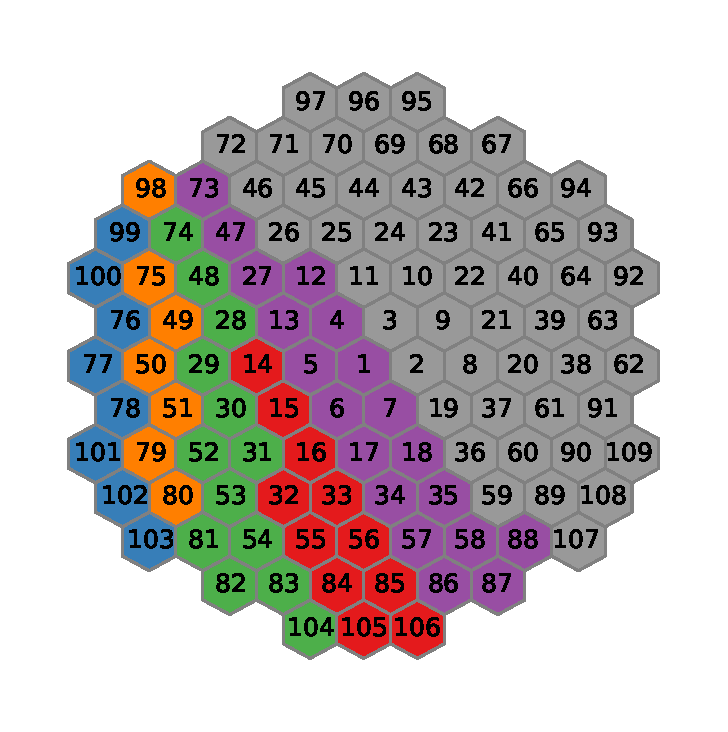
\includegraphics[width=0.35\textwidth]{2012-3_retina_all.pdf}
    \caption{The SPHERE-2 PMT mosaic scheme. PMT numbers are indicated. PMTs are colored according to their current curve type in the 2012-3 flight with colors as in Figure~\ref{fig:2012-3_currents}.}
    \label{fig:2012-3_shore_image}
\end{figure}
%%%%%%%%%%%%%%%%%%%%%%%%%%%%%

However, in the third flight of the 2012 season in part of the PMTs an abnormal drop in the currents was observed.
%(see Figure~\ref{fig:2012-3_currents}).
The registered currents from some of the PMTs (numbers 5, 14, 29, 50 and 77) are shown in Figure~\ref{fig:2012-3_currents}, top panel. These PMTs form a straight line on the PMT mosaic and the currents dropped and restored in them in the same order as they are positioned. This behaviour was observed for a number of PMTs with current drops occurring at the same time. In Figure~\ref{fig:2012-3_shore_image} the PMTs are colored according to similar patterns in the current drop and restore times.

This anomaly was observed in the first half of the flight during observations made at an altitude of 850~m. At that time according to the GPS the balloon was drifting north from the starting point. Detector altitude and drift are shown in Figure~\ref{fig:2012-3_currents}, central panel. Due to wind strengthening at that altitude the balloon was subsequently lowered to 480~m and the currents returned to their normal behaviour. 

Analysis of the detector position and tilt showed that at that time it was observing a part of the shoreline and land surface. At this location the shoreline is a narrow artificial ledge built for the railroad and further changes into a steep snowless cliff wall with trees atop (see Figure~\ref{fig:2012--shore-view}). The reflective properties of both rock and pine trees is way lower than that of snow. In Figure~\ref{fig:2012-drift} the detector trajectory (green line) and starting point (purple cross) are given. The detector position (blue cross) and corresponding PMT centers projections onto the surface are given for time point 15:47 UTC with the detector inclination of 8$^\circ$ to the north, the moment of the highest current drop and furthest drift towards the shore.The behavior of the currents in each PMT is consistent with its crossing of the shoreline. The PMTs that show no drop in their currents by our estimations always observe a clear snow covered surface of the lake. In all other flights no instances of detector drift to the shore was observed. 

This observation itself confirms the consistency of the detector orientation and position monitoring.

\section{Telemetry analysis}

The position and inclination of the SPHERE-2 detector are important values for the correct reconstruction of the Cherenkov light characteristics of registered EAS. In contrast to Cherenkov ground-based arrays, such as~\cite{Yakutsk19,TUNKA133}, the SPHERE-2 detector has a variable registration area depending on both altitude and inclination.

%%%%%%%%%%%%%%%%%%%%%%%%%%%%%%%%%%%%%%%%%%%%%%%%%%%
\subsection{GPS altitude correction with barometer data}
\label{sect:gps_correction}

Thorough telemetry data analysis revealed that at several periods of time the recorded altitude from the GPS data was inadequate. Namely, after rapid changes in altitude due to the balloon ascent or descent the GPS registered height lagged behind from the corresponding pressure change and varied in a smoothed fashion. The example of such behavior is shown in Figure~\ref{fig:h_corr}, top panel. We were unable to pin the exact source of this distortion, but our best guess is that it's the result of the GPS module's internal error correction algorithm. The module's primary application is for naval/aerial navigation~\cite{GPS-module-specs} and it might be interpreting sudden changes in altitude without a proper horizontal speed as an error.

\begin{figure}[tb]
    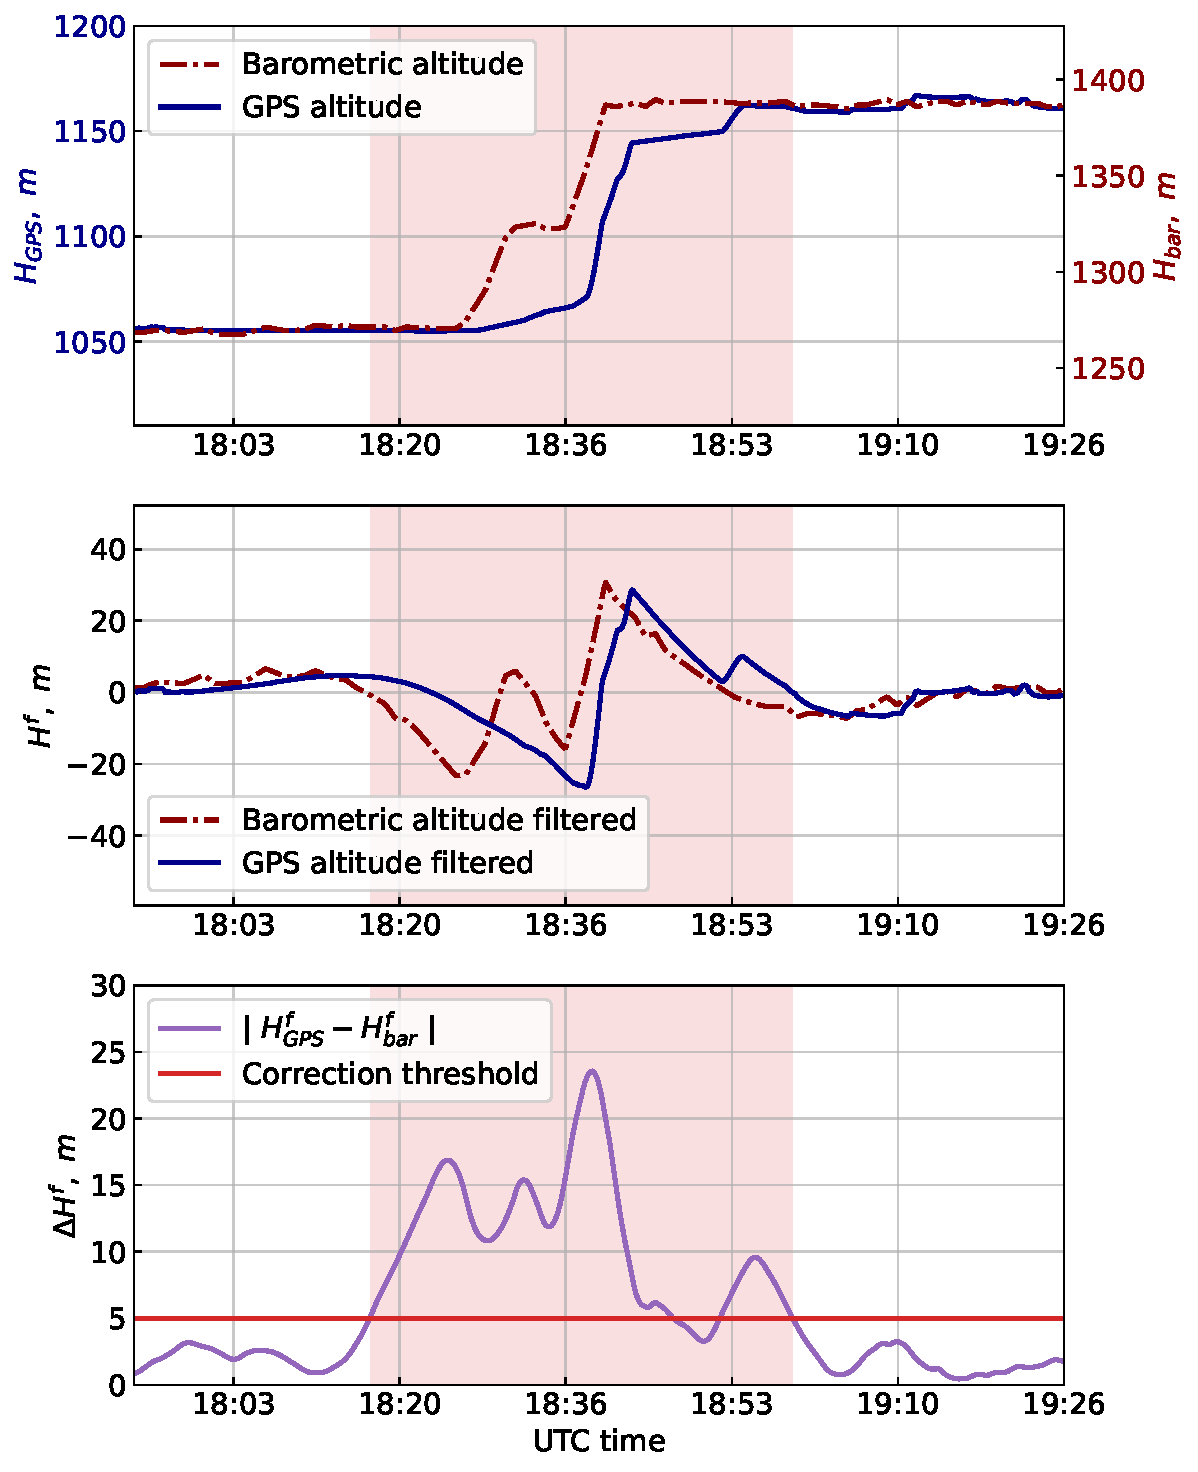
\includegraphics[width=0.48\textwidth]{figs/2013-2_gps_correction.pdf} 
    \caption{An example of the anomalous GPS altitude behavior, as compared with the `barometric' altitude (top panel) during flight 2013-2. Same data with a high-pass digital Butterworth filter applied (middle panel). Smoothed absolute delta of high-passed altitudes from the middle panel, used as a gate with the threshold set by the red line; intervals above this line correspond to the red bands on the other panels, which are the intervals subjected to GPS data correction.}
\label{fig:h_corr}
\end{figure}

Time intervals where GPS data exhibit this behaviour are relatively short for most flights, but some events were recorded during them. In order to correctly estimate the detector altitude for those events, and to maintain the overall data consistency we attempted to correct these smoothed GPS altitude measurements using the pressure data from the barometer, which has a strong dependence on the altitude.

To identify the affected time intervals we calculated the approximate `barometric height' $H_{bar}$ from the pressure data using the inverted barometric formula $H_{bar} = H_0 - a \log (P/P_0)$ with following parameters: $H_0 = 456~\textrm{m}$ (Baikal lake surface level), $P_0 = 1000~\textrm{hPa}$ (close to average March pressure on the Baikal surface) and $a = {RT}/{Mg} \approx 8400~\textrm{m}$ (standard value for the barometric formula). In reality this value gives only a rough approximation to the real altitude as pressure is affected by many atmospheric conditions (temperature, humidity, wind). To compare $H_{bar}$ with GPS-measured altitude $H_{GPS}$ we applied a high-pass digital Butterworth filter to both values, which yields only the fast fluctuations of both values and removes slowly drifting baseline values. The cutoff for the filter was set to $T=40~\textrm{min}$ ($0.416~\textrm{mHz}$) and slope to $12~\textrm{db per octave}$. The filtered data $H_{GPS}^{\textrm{f}}$ and $H_{bar}^{\textrm{f}}$ is shown on Figure~\ref{fig:h_corr}, middle panel.

During stable altitude periods $H_{GPS}^{\textrm{f}}$ and $H_{bar}^{\textrm{f}}$ are subject to fast, somewhat correlated fluctuations. In contrast, intervals of anomalous GPS data correspond to a divergence of these two values. Hence, we used the absolute difference $|H_{GPS}^{\textrm{f}} - H_{bar}^{\textrm{f}}|$ as an indicator for anomalous behaviour. To increase the robustness of the indication we have also applied the moving average (MA) smoothing with a $6~\textrm{min}$ window, so that fast relative fluctuations of GPS altitude and pressure do not indicate the anomaly. The threshold for the indicator was chosen to be $5~\textrm{m}$. The example of the indicator value $\Delta H^\textrm{f}$ = $\textrm{MA}(|H_{GPS}^{\textrm{f}} - H_{bar}^{\textrm{f}}|)$ is shown on Figure~\ref{fig:h_corr}, bottom panel, and the indicator threshold is shown in horizontal red line. The correction interval chosen based on the indicator and the threshold is shown on all panels as a vertical pink band.

After the anomalous intervals were identified, for each of them we picked two adjacent $3~\textrm{min}$ intervals with correct GPS data. If two anomalous intervals were closer than $3~\textrm{min}$ in time they were merged together (this behaviour is seen on Figure~\ref{fig:h_corr} in the fact that the short non-anomalous (the indicator is below the threshold) interval around 18:40 is included in the large pink band. With these intervals of valid GPS altitude and pressure data we have performed an interpolated altitude in the anomalous interval with 'local' barometric formula with parameters $a$ and $P_0$ fitted to the data.

The correction was made for the total of 220 minutes of all flights. During this time around 68 triggers were registered. The total distribution of the time spent by the detector at each height is presented in Figure~\ref{fig:time_on_altitude}. Most of the time the detector spent at 400, 500, 580 and 890~m. However, the actual distribution of the registered events across the altitudes is a more complex question since the trigger settings and overall detector performance changed over time and across seasons. Careful analysis of this question will be covered in following publications.

\begin{figure}[tb]
    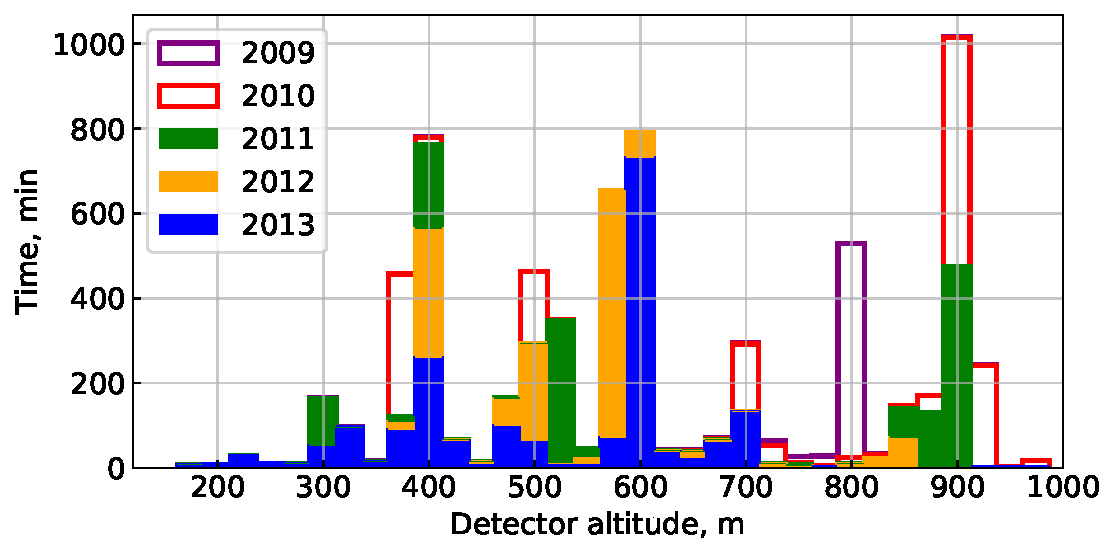
\includegraphics[width=19pc]{figs/time_on_altitude_c.pdf}%
    \caption{Altitude distribution over the experiment time.}
    \label{fig:time_on_altitude}
\end{figure}

%%%%%%%%%%%%%%%%%%%%%%%%%%%%%%%%%
%%% Atmosphere profiles figures %%%%
\begin{figure*}[tb]
    \begin{minipage}[t]{0.48\textwidth}
       \centering
       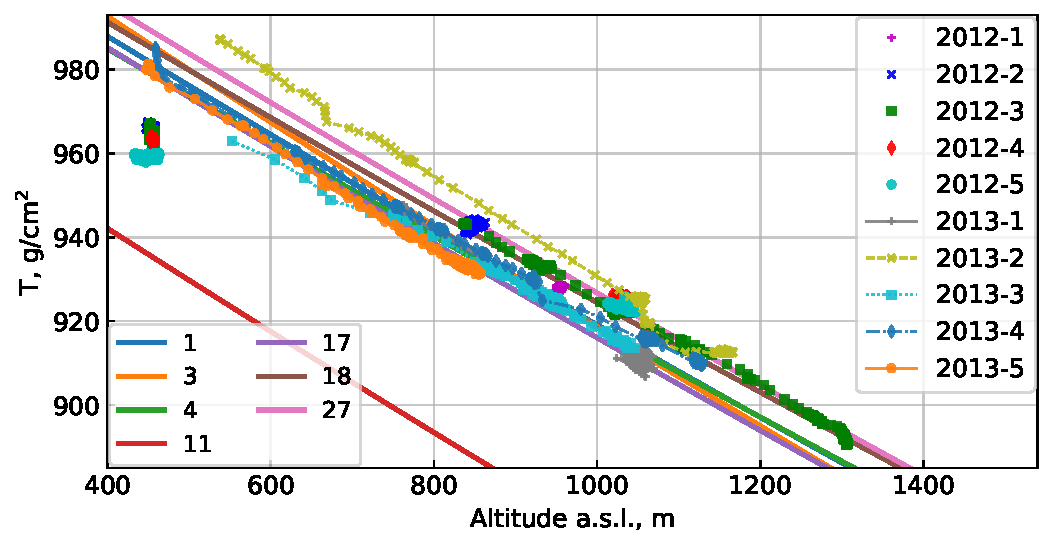
\includegraphics[width=\textwidth]{figs/atmosphere_T.pdf}
       \caption{Mass overburden versus altitude experimental data (points) in each flight and CORSIKA profiles (solid lines with corresponding model numbers). For preliminary SPHERE-2 modeling and analysis the N0 11 atmosphere was used.}
        \label{fig:massoverburden}
    \end{minipage}
    \hfill
    \begin{minipage}[t]{0.48\textwidth}
        \centering
        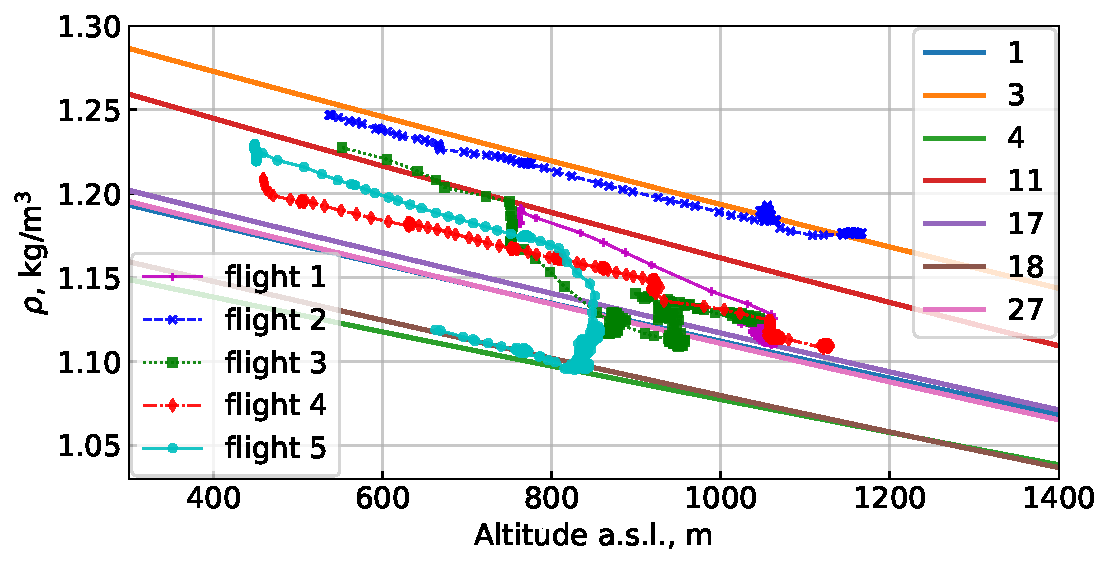
\includegraphics[width=\textwidth]{figs/atmosphere_rho.pdf}
        \caption{Density versus altitude experimental data (points) in each flight and CORSIKA model density profiles (solid lines) same as in Figure \ref{fig:massoverburden}).}
        \label{fig:density}
   \end{minipage}
\end{figure*}
%%%%%%%%%%%%%%%%%%%%%%%%%%%%%%%%%


\subsection{Atmosphere density profile}
\label{sect:atmosphere-profile}

After the corrections were applied to GPS altitudes the atmosphere density profiles were reconstructed. Direct measurements with an on-board barometer and thermometer were taken only at altitudes below 900~m above the ice, therefore information about higher atmospheric conditions is not available. To obtain the best extrapolation of this data we had to use a set of parameterized atmospheres provided by the CORSIKA software~\cite{hec98} version 7.5600.

In CORSIKA the atmosphere is described in terms of mass overburden $t(H)$ that is parameterized as a piecewise continuous function which has exponential behavior in the lower four layers and linear in the highest one. CORSIKA code provides 26 atmosphere models corresponding to measurements taken at different seasons in different locations around the globe. For each model of the atmosphere our experimental data was fully located in the lowest layer.

We used the following equations to derive the mass overburden $t$ and density $\rho$ from the measured pressure $p$ and temperature~$T$ data.

\begin{equation}
t     = \frac{p}{g}, \\ \hspace{7pt}
\rho  = \frac{p \, M}{R \, T} \\
\end{equation}


Here $g$ is the gravitational acceleration, $M$ is the average molar mass of air, $R$ is the gas constant.

Mass overburden data was reconstructed from atmospheric pressure measurements and air density was estimated based on both air pressure and temperature around the balloon. Calculated experimental points for $t$ and $\rho$ for each flight are shown in Figure~\ref{fig:massoverburden} and Figure~\ref{fig:density} respectively. CORSIKA atmospheres are shown with solid lines. The profile that was adopted prior to the actual measurements for the preliminary modeling (atmosphere model 11) is shown by the red line. From this comparison it may be seen that the previously picked atmosphere is inconsistent with our experimental data for $t$ in terms of absolute values, but their derivatives lie relatively close. 
%Therefore either a full remodeling with a better fitting atmosphere or some corrections in the final data are required to reduce the systematic errors in energy and composition estimations.



%%%%%%%%%%%%%%%%%%%%%%%%%%%%%%%%%
%%% === Table CORSIKA
\begin{table}[tbh]
\centering
\caption{Total Cherenkov photons numbers ratios for different CORSIKA atmosphere model pairs: means, variations, relative variations given for 10 PeV primary protons. Zenith angle 15$^\circ$. Sample volume 30 events.}
\label{tab:atmmod}
%\vspace{1pc}
\begin{tabular}{cccc}
    \toprule
    model/primary   & mean &  variation   & relative variation \\ 
         pair       &  $m$ & $\sigma$     & $\sigma/m$ \\ 
    \midrule 
     3/4 &  1.015     &  0.0490     &   0.0483   \\
    11/3 &  0.9834    &  0.0511     &   0.0520   \\
    11/4 &  0.9963    &  0.0443     &   0.0445   \\
    \midrule
     p/Fe &  1.232     &  0.0686     &   0.0557   \\
    \bottomrule
\end{tabular}
\end{table}
%%%%%%%%%%%%%%%%%%%%%%%%%%%%%%%%%


%%%%%%%%%%%%%%%%%%%%%%%%%%%%%%%%%
%%% === LDF Calculation
\begin{figure*}[tb]
    \begin{minipage}[t]{0.48\textwidth}
        \centering
        %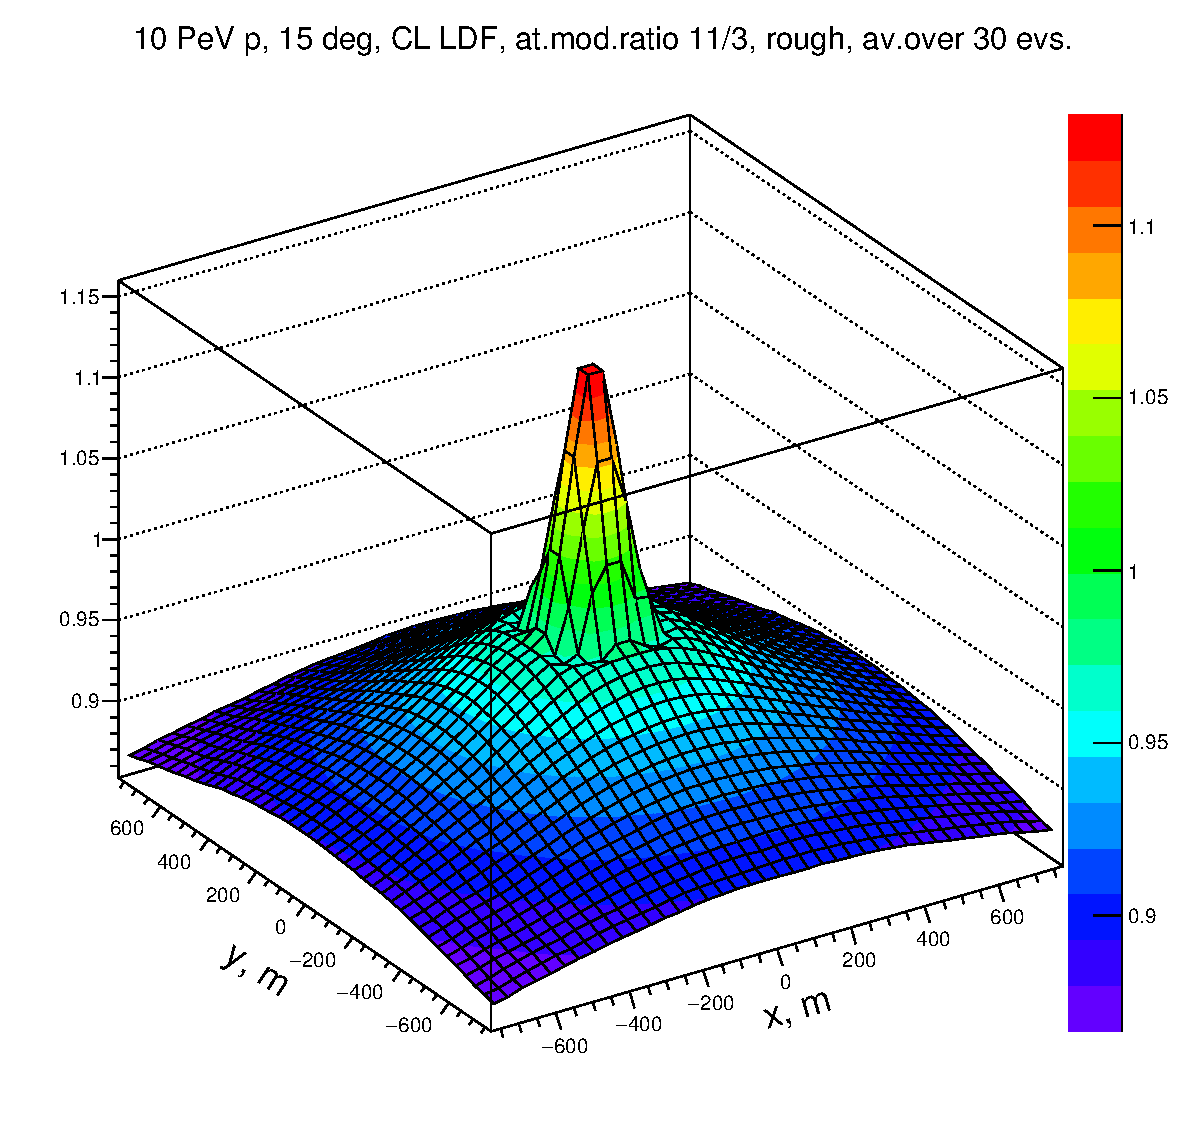
\includegraphics[width=19pc]{11d3}%
        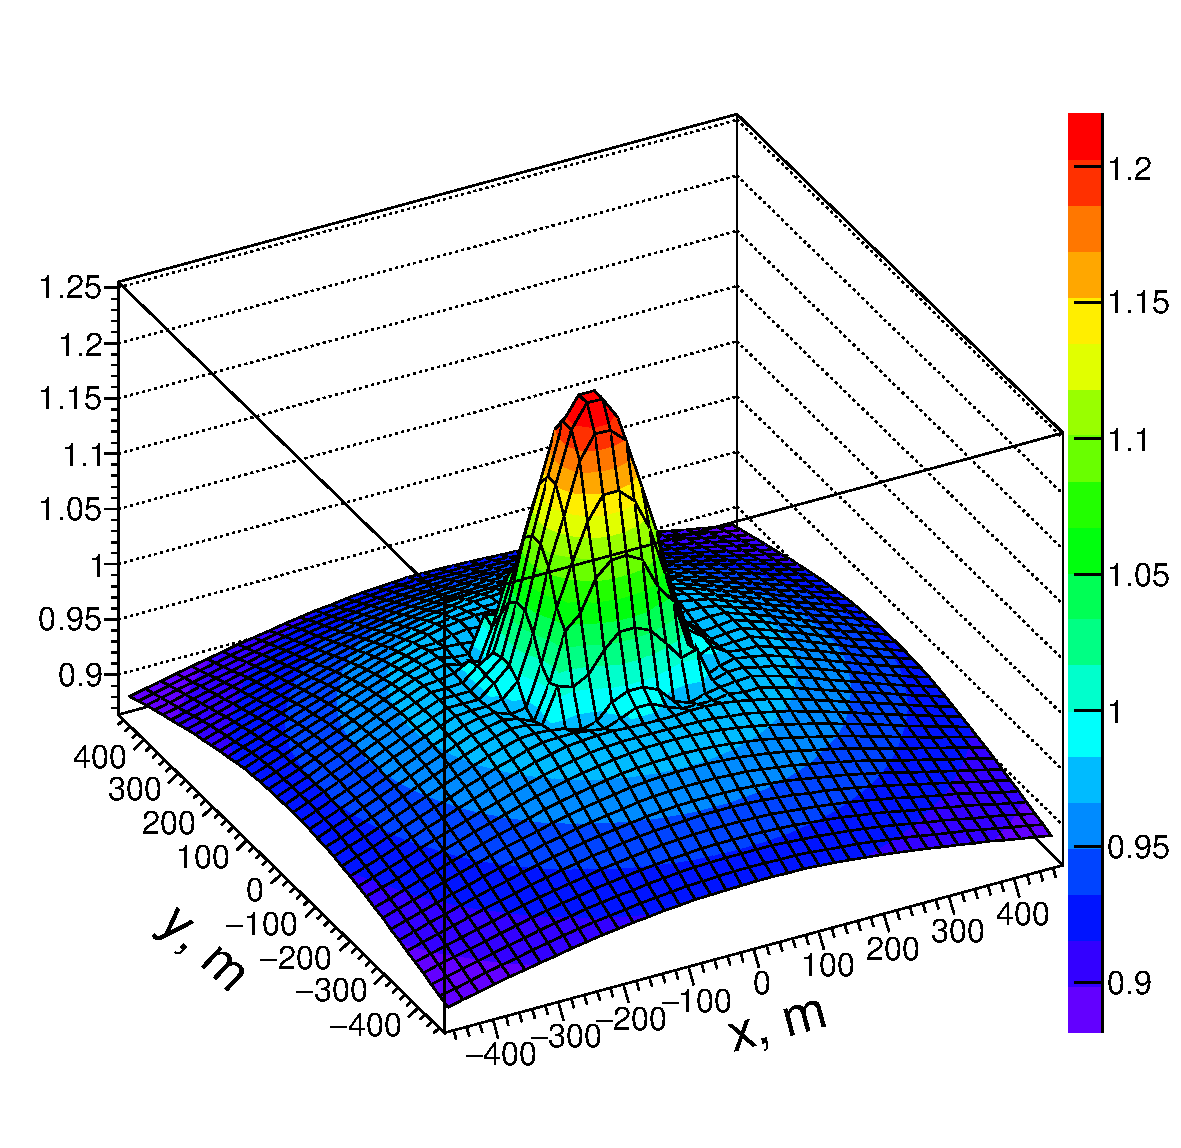
\includegraphics[width=19pc]{10PeV_pro_15deg_m11_over_m04}%
        \vspace{-1.0pc}
        \caption{The ratio of sample averaged Cherenkov photons distribution for the CORSIKA atmosphere model pair 11/4. Bin size 50~m $\times$ 50~m. Primary protons with 10~PeV energy. Zenith angle 15$^\circ$. Sample volume 30~events.}
        \label{fig:4d11}
    \end{minipage}
    \hfill
    \begin{minipage}[t]{0.48\textwidth}
        \centering
        %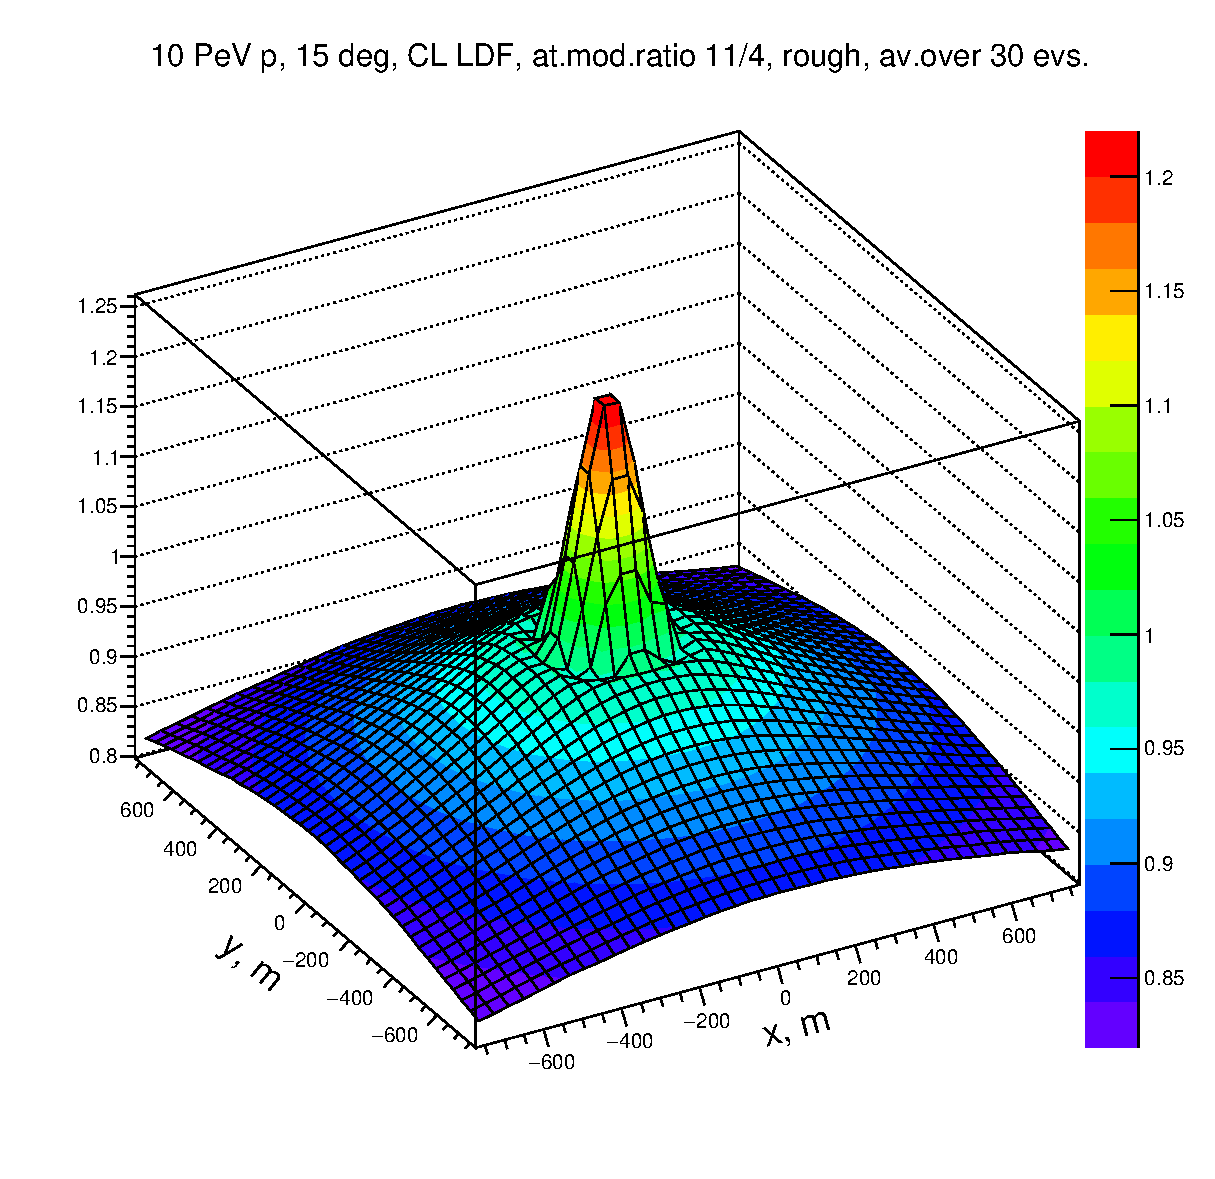
\includegraphics[width=19pc]{11d4}%
        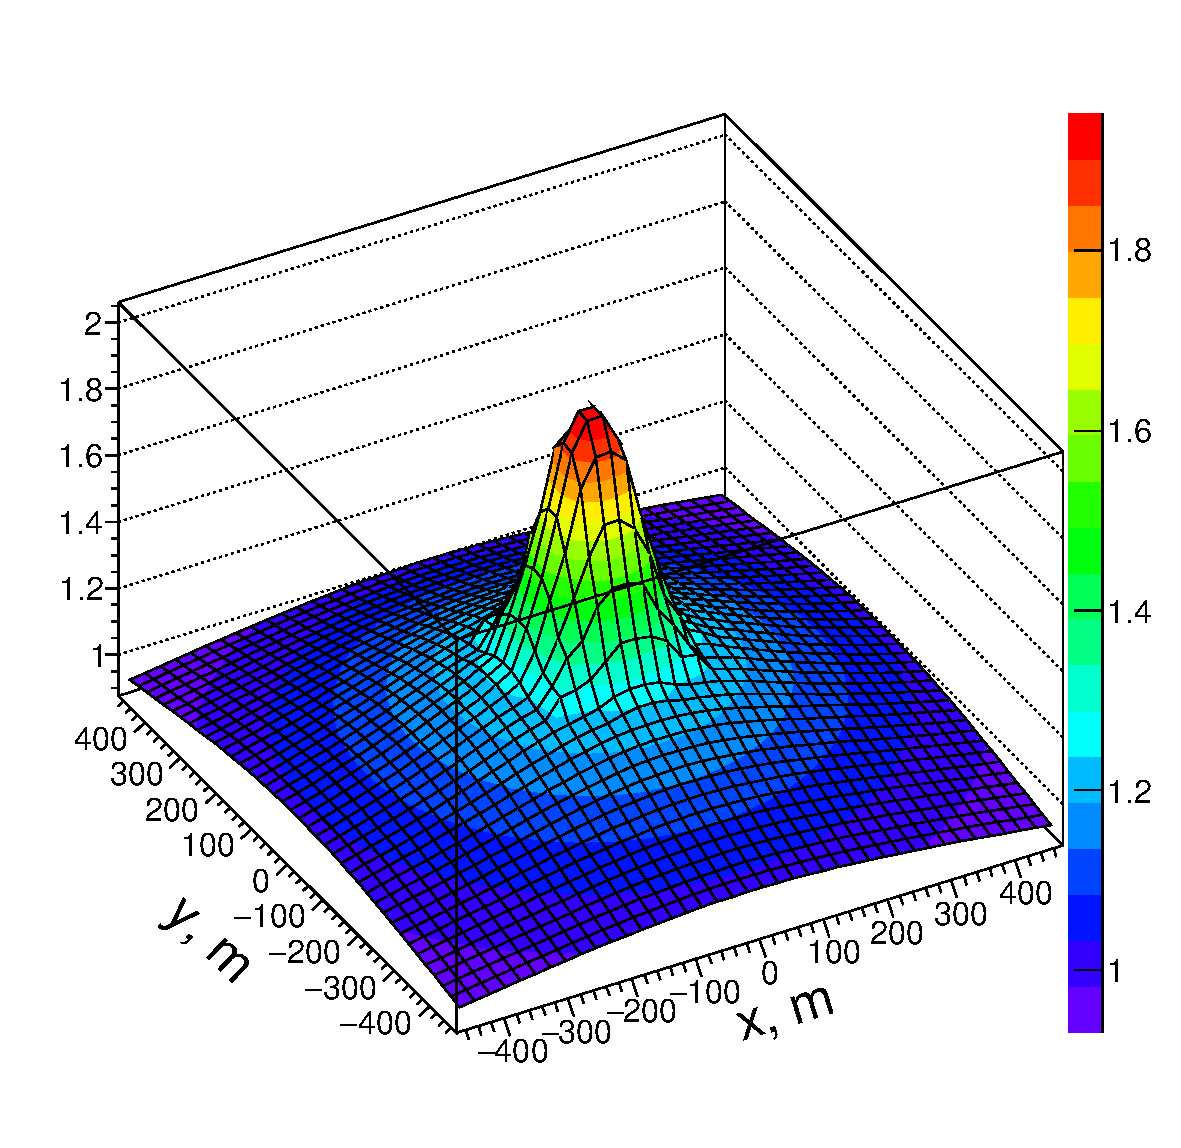
\includegraphics[width=19pc]{10PeV_15deg_pro_over_Fe}%
        \vspace{-1.0pc}
        \caption{The ratio of sample averaged Cherenkov photons distribution for the nuclear pair proton/Fe for the CORSIKA atmosphere model 11. Bin size 50~m $\times$ 50~m. Primary protons with 10~PeV energy. Zenith angle 15$^\circ$. Sample volume 30~events.}
        \label{fig:pdFe}
    \end{minipage}
\end{figure*}
%%%%%%%%%%%%%%%%%%%%%%%%%%%%%%%%%

%\begin{paracol}{2}

CORSIKA atmosphere model 11 was selected based on available monthly averages from Irkutsk airport weather station located 70 km to the North of the balloon launch site. The model was used for preliminary modelling and estimations at the experiment planning stage. However, our data show that this choice was not ideal.

The use of experimental points in $t$ or $\rho$ cannot provide a reasonable choice of the model, but only give a clue as to what the model should be. A full-fledged choice must include data on the vertical profile of the atmosphere up to altitudes of at least 10 km above the lake because Cherenkov light mostly comes from this layer. Still some conclusions on the atmosphere model effect on primary energy and mass estimates can be made by comparing the artificial showers simulated for different models.

Artificial showers initiated by 10~PeV protons were modeled using CORSIKA for atmosphere model 11 resembling the experimental $\rho$ curves, as well as for models 3 and 4 roughly following the data on $t$. The results are expressed as total numbers of Cherenkov photons in a shower and Cherenkov photons distributions on an observation level. We use primary proton showers here because they reveal the most pronounced atmosphere model effect since proton showers exhibit the largest fluctuations in their development. Sometimes proton-induced showers even behave like iron-induced ones in both longitudinal profiles and  Cherenkov light distributions. 

The Cherenkov photons distributions were calculated within a vast carpet (3.2~km $\times$ 3.2~km) tiled with 2.5~m~$\times$~2.5~m squares but for the purpose of comparison were smoothed by integrating over 50~m~$\times$~50~m squares approximately imitating the sensitivity spots of the telescope pixels at the 0.5 km altitude.

The sample volume was 30 sets of 3 showers each. The showers in each set used the same random seeds but different atmosphere models (CORSIKA models No 3, 4 and 11) for each shower. The same random seeds were used in order to diminish the effect of shower longitudinal development variations. The total number of Cherenkov photons for each shower were used to form a set of individual total Cherenkov photon number ratios: pairs 3 to 4, 3 to 11 and 4 to 11. Table~\ref{tab:atmmod} shows the mean values and variations of these ratios. For the reference in the last row of the Table the ratio is given for the same atmosphere model No~11 but for different primaries (proton to iron). Here again individual showers modeled with the same random seeds but different primaries were used to form a ratio. 

Figure~\ref{fig:4d11} shows the ratio of averaged Cherenkov photons distribution modelled for atmosphere No~11 to averaged Cherenkov photons distribution modelled for atmosphere No~4. Figure~\ref{fig:pdFe} shows the same ratio of the average Cherenkov photons distributions of proton-induced and iron-induced showers for the atmosphere model 11 to demonstrate the scale of the primary mass effect.

%Pair 3/4 reflects the maximal effect of the atmosphere model from the viewpoint of experimental $t$ and $\rho$ measurements. Pairs 3/11 and 4/11 compare model 11 used for simulations to the models approximating the experimental data.

Table data clearly states that substantial changes of the atmosphere model affect the total number of Cherenkov photons and, therefore, the estimates of primary energy by no more than 5\% on average. Conclusions on primary mass estimates are not as clear, but the Cherenkov photons distribution ratio plots indicate the changes in Cherenkov photons distributions to be about 6 to 12\% (12 to 20\%) near the shower core, closer than 80 m, and about -2 to +6\% (0 to +12\%) in the 80--150m circle for the 3/11 (4/11) pair, which definitely affects our mass-sensitive criterion described in~\cite{Ant15c}. Our preliminary studies indicate that the mass-sensitive parameter based on the Cherenkov light lateral distribution function steepness is extremely sensitive to the atmosphere model. In the case of the parameter used in our study the value of the parameter varies greater with atmosphere than with primary particle mass. The good knowledge of the atmosphere parameters is crucial to the reliable primary particle mass estimation.

The detailed description of our primary particle mass estimation procedure with accurate evaluation of the atmospheric effects and related uncertainties will be given elsewhere. 


\section{Conclusions \label{sect:conclusions}}
The SPHERE-2 detector which operated in 2008--2013 had a large array of supplementary sensors that allowed to control and later reconstruct the state of the detector and measurement conditions. 

For the reflected Cherenkov light method the information on detector position and orientation is vital. Their values were measured with good precision and reliability and were cross-checked using experimental data.

Measurements of air pressure and temperature during flights gave information on the atmospheric state that will allow to introduce different atmospheric models into analysis and to account their strong impact on the results. Availability of the data on the atmospheric state at the moment of the EAS detection allows higher primary mass reconstruction. Carrying out daily measurements of the state of the atmosphere in different layers of the atmosphere is critical for reconstructing the composition of cosmic rays. This is important not only for balloons, but also for ground based installations.


  
\acknowledgments{
We are grateful to the Lebedev Physical Institute of the Russian Academy of Sciences group (leader S.B.~Shaulov) for assistance in assembling and testing the electronic equipment and in preparation of expeditions. We also thank the Baikal-GVD collaboration and G.V.~Domogatsky (Institute for Nuclear Research, Russian Academy of Sciences) for the support of the SPHERE experiment at the Baikal Lake scientific station.}

\funding{M. Finger and M. Finger Jr. were supported by MEYS of Czech Republic grants LG14004 and LG18022.}

\end{paracol}

\reftitle{References}
%\section{References}
%=====================================
% References, variant A: external bibliography
%=====================================
\externalbibliography{yes}
%\bibliography{your_external_BibTeX_file}
\bibliography{Sphere-Data.bib}
\end{document}